%% BioMed_Central_Tex_Template_v1.06
%%                                      %
%  bmc_article.tex            ver: 1.06 %
%                                       %

%%IMPORTANT: do not delete the first line of this template
%%It must be present to enable the BMC Submission system to
%%recognise this template!!

%%%%%%%%%%%%%%%%%%%%%%%%%%%%%%%%%%%%%%%%%
%%                                     %%
%%  LaTeX template for BioMed Central  %%
%%     journal article submissions     %%
%%                                     %%
%%          <8 June 2012>              %%
%%                                     %%
%%                                     %%
%%%%%%%%%%%%%%%%%%%%%%%%%%%%%%%%%%%%%%%%%

%%%%%%%%%%%%%%%%%%%%%%%%%%%%%%%%%%%%%%%%%%%%%%%%%%%%%%%%%%%%%%%%%%%%%
%%                                                                 %%
%% For instructions on how to fill out this Tex template           %%
%% document please refer to Readme.html and the instructions for   %%
%% authors page on the biomed central website                      %%
%% http://www.biomedcentral.com/info/authors/                      %%
%%                                                                 %%
%% Please do not use \input{...} to include other tex files.       %%
%% Submit your LaTeX manuscript as one .tex document.              %%
%%                                                                 %%
%% All additional figures and files should be attached             %%
%% separately and not embedded in the \TeX\ document itself.       %%
%%                                                                 %%
%% BioMed Central currently use the MikTex distribution of         %%
%% TeX for Windows) of TeX and LaTeX.  This is available from      %%
%% http://www.miktex.org                                           %%
%%                                                                 %%
%%%%%%%%%%%%%%%%%%%%%%%%%%%%%%%%%%%%%%%%%%%%%%%%%%%%%%%%%%%%%%%%%%%%%

%%% additional documentclass options:
%  [doublespacing]
%  [linenumbers]   - put the line numbers on margins

%%% loading packages, author definitions

%\documentclass[twocolumn]{bmcart}% uncomment this for twocolumn layout and comment line below
\documentclass{bmcart}

%%% Load packages
%\usepackage{amsthm,amsmath}
% \RequirePackage{natbib}
\RequirePackage[authoryear]{natbib}% uncomment this for author-year
% bibliography
%\RequirePackage{hyperref}
%\usepackage[utf8]{inputenc} %unicode support
%\usepackage[applemac]{inputenc} %applemac support if unicode package fails
%\usepackage[latin1]{inputenc} %UNIX support if unicode package fails

%%%%%%%%%%%%%%%%%%%%%%%%%%%%%%%%%%%%%%%%%%%%%%%%%%%%%%%%%%%%%%%%%%%%%%%%
% preamble from authors
\usepackage{amsmath}
\usepackage{amsthm}
%\usepackage{appendix}
%\usepackage{amssymb} % for approx greater than
%\usepackage{caption}
\usepackage{placeins} % for \FloatBarrier
\usepackage{graphicx}
\usepackage{subcaption}
\usepackage{longtable}
\usepackage{setspace}
\usepackage{booktabs}
\usepackage{tabularx}
%\usepackage{xcolor,colortbl}
\usepackage{chngpage}
%\usepackage{natbib}
%\bibpunct{(}{)}{,}{a}{}{;} 
\usepackage{url}
\usepackage{nth}
%\usepackage{authblk}
%\usepackage[most]{tcolorbox}
\usepackage[normalem]{ulem}
\usepackage{amsfonts}
% columns for longtable. These work if floats not being
% pushed to end!! commented out to remove compile error
\newcolumntype{C}[1]{>{\centering\let\newline\\\arraybackslash\hspace{0pt}}m{#1}}
\newcolumntype{L}[1]{>{\raggedright\let\newline\\\arraybackslash\hspace{0pt}}m{#1}}
\usepackage{arydshln} % Dashed lines in matrices
\usepackage{lastpage}
%\usepackage[margin=1in]{geometry}
%\doublespacing % for review

%%%%%%%%%%%%%%%%%%%%%%%%%%%%%%%%%%%%%%%%%%%%%%%%%%%%%%%%%%%%%%%%%%%%%%%%%%%%%
% places figures and tables at end. Required for review guidelines!!!
%\usepackage[nolists, nomarkers]{endfloat}
%\DeclareDelayedFloatFlavor{longtable}{table}
%\renewcommand{\efloatseparator}{\mbox{}} % This removes pagebreaks
%%%%%%%%%%%%%%%%%%%%%%%%%%%%%%%%%%%%%%%%%%%%%%%%%%%%%%%%%%%%%%%%%%%%%%%%%%%%%%
% for section 4 math environments
\theoremstyle{definition}
\newtheorem{definition}{Definition}[section]
\newtheorem{theorem}{Theorem}[section]
\newtheorem{proposition}{Proposition}[section]
\newtheorem{corollary}{Corollary}[proposition]
\newtheorem{remark}{Remark}[section]

%%%%%%%%%%%%%%%%%%%%%%%%%%%%%%%%%%%%%%%%%%%%%%%%%%%%%%%%%%%%%%%%%%%%%%%%%%%%%%

\newcommand\ackn[1]{%
  \begingroup
  \renewcommand\thefootnote{}\footnote{#1}%
  \addtocounter{footnote}{-1}%
  \endgroup
}

%%%%%%%%%%%%%%%%%%%%%%%%%%%%%%%%%%%%%%%%%%%%%%%%%%%%%%%
% functions to read in table elements for timelines and graphs table in sec 4 (table 3)
\newcommand{\ttt}[2]{\includegraphics[scale=.45]{{Tab3#1#2}.pdf}}

% Affiliations in small font size
%\renewcommand\Affilfont{\small}

%\defcitealias{HMD}{HMD 2014}

% junk for longtable caption
%\AtBeginEnvironment{longtable}{\linespread{1}\selectfont}
%\setlength{\LTcapwidth}{\linewidth}

% sort van Raalte properly
% #1: sorting key, #2: prefix for citation, #3: prefix for bibliography
\DeclareRobustCommand{\VAN}[3]{#2} % set up for citation

%%%%%%%%%%%%%%%%%%%%%%%%%%%%%%%%%%%%%%%%%%%%%%%%%
%%                                             %%
%%  If you wish to display your graphics for   %%
%%  your own use using includegraphic or       %%
%%  includegraphics, then comment out the      %%
%%  following two lines of code.               %%
%%  NB: These line *must* be included when     %%
%%  submitting to BMC.                         %%
%%  All figure files must be submitted as      %%
%%  separate graphics through the BMC          %%
%%  submission process, not included in the    %%
%%  submitted article.                         %%
%%                                             %%
%%%%%%%%%%%%%%%%%%%%%%%%%%%%%%%%%%%%%%%%%%%%%%%%%


%\def\includegraphic{}
%\def\includegraphics{}



%%% Put your definitions there:
\startlocaldefs
\endlocaldefs

%%% Begin ...
\begin{document}

%%% Start of article front matter
\begin{frontmatter}

\begin{fmbox}
\dochead{Research}

%%%%%%%%%%%%%%%%%%%%%%%%%%%%%%%%%%%%%%%%%%%%%%
%%                                          %%
%% Enter the title of your article here     %%
%%                                          %%
%%%%%%%%%%%%%%%%%%%%%%%%%%%%%%%%%%%%%%%%%%%%%%

\title{A unified framework of demographic time}

%%%%%%%%%%%%%%%%%%%%%%%%%%%%%%%%%%%%%%%%%%%%%%
%%                                          %%
%% Enter the authors here                   %%
%%                                          %%
%% Specify information, if available,       %%
%% in the form:                             %%
%%   <key>={<id1>,<id2>}                    %%
%%   <key>=                                 %%
%% Comment or delete the keys which are     %%
%% not used. Repeat \author command as much %%
%% as required.                             %%
%%                                          %%
%%%%%%%%%%%%%%%%%%%%%%%%%%%%%%%%%%%%%%%%%%%%%%

\author[
   %addressref={aff1},                   % id's of addresses, e.g. {aff1,aff2}
   %corref={aff1},                       % id of corresponding address, if any
   %noteref={n1},                        % id's of article notes, if any
   %email={jane.e.doe@cambridge.co.uk}   % email address
]{\fnm{[authors blinded]}}%\inits{JE}\fnm{Jane E} \snm{Doe}}
%\author[
%%   addressref={aff1,aff2},
%   email={john.RS.Smith@cambridge.co.uk}
%]{\inits{JRS}\fnm{John RS} \snm{Smith}}

%%%%%%%%%%%%%%%%%%%%%%%%%%%%%%%%%%%%%%%%%%%%%%
%%                                          %%
%% Enter the authors' addresses here        %%
%%                                          %%
%% Repeat \address commands as much as      %%
%% required.                                %%
%%                                          %%
%%%%%%%%%%%%%%%%%%%%%%%%%%%%%%%%%%%%%%%%%%%%%%

%\address[id=aff1]{%                           % unique id
%  \orgname{Department of Zoology, Cambridge}, % university, etc
%  \street{Waterloo Road},                     %
%  %\postcode{}                                % post or zip code
%  \city{London},                              % city
%  \cny{UK}                                    % country
%}
%\address[id=aff2]{%
%  \orgname{Marine Ecology Department, Institute of Marine Sciences Kiel},
%  \street{D\"{u}sternbrooker Weg 20},
%  \postcode{24105}
%  \city{Kiel},
%  \cny{Germany}
%}

%%%%%%%%%%%%%%%%%%%%%%%%%%%%%%%%%%%%%%%%%%%%%%
%%                                          %%
%% Enter short notes here                   %%
%%                                          %%
%% Short notes will be after addresses      %%
%% on first page.                           %%
%%                                          %%
%%%%%%%%%%%%%%%%%%%%%%%%%%%%%%%%%%%%%%%%%%%%%%

\begin{artnotes}
%\note{Sample of title note}     % note to the article
\note[id=n1]{Equal contributor} % note, connected to author
\end{artnotes}

\end{fmbox}% comment this for two column layout

%%%%%%%%%%%%%%%%%%%%%%%%%%%%%%%%%%%%%%%%%%%%%%
%%                                          %%
%% The Abstract begins here                 %%
%%                                          %%
%% Please refer to the Instructions for     %%
%% authors on http://www.biomedcentral.com  %%
%% and include the section headings         %%
%% accordingly for your article type.       %%
%%                                          %%
%%%%%%%%%%%%%%%%%%%%%%%%%%%%%%%%%%%%%%%%%%%%%%

\begin{abstractbox}

\begin{abstract} % abstract
Demographic thought and practice is largely conditioned by the Lexis diagram,
a two-dimensional graphical representation of the identity between age,
period, and birth cohort. This relationship does not account for remaining years
of life, total length of life, or time of death, whose use in
demographic research is both underrepresented and incompletely situated. We
describe an identity between these six demographic time measures and describe
the sub-identities and diagrams that pertain to this identity. We provide an
application of this framework to the measurement of late-life morbidity prevalence. We generalize these relationships to higher order identities derived from an
arbitrary number of events in calendar time. Our examples are based on
classic human demography, but the concepts we present can reveal patterns and
relationships in any event history data, and contribute to the study of human or
non-human population dynamics measured on any scale of calendar time.
\end{abstract}

%%%%%%%%%%%%%%%%%%%%%%%%%%%%%%%%%%%%%%%%%%%%%%
%%                                          %%
%% The keywords begin here                  %%
%%                                          %%
%% Put each keyword in separate \kwd{}.     %%
%%                                          %%
%%%%%%%%%%%%%%%%%%%%%%%%%%%%%%%%%%%%%%%%%%%%%%

\begin{keyword}
\kwd{age structure}
\kwd{formal demography}
\kwd{data visualization}
\kwd{age period cohort}
\end{keyword}

% MSC classifications codes, if any
%\begin{keyword}[class=AMS]
%\kwd[Primary ]{}
%\kwd{}
%\kwd[; secondary ]{}
%\end{keyword}

\end{abstractbox}
%
%\end{fmbox}% uncomment this for twcolumn layout

\end{frontmatter}

%%%%%%%%%%%%%%%%%%%%%%%%%%%%%%%%%%%%%%%%%%%%%%
%%                                          %%
%% The Main Body begins here                %%
%%                                          %%
%% Please refer to the instructions for     %%
%% authors on:                              %%
%% http://www.biomedcentral.com/info/authors%%
%% and include the section headings         %%
%% accordingly for your article type.       %%
%%                                          %%
%% See the Results and Discussion section   %%
%% for details on how to create sub-sections%%
%%                                          %%
%% use \cite{...} to cite references        %%
%%  \cite{koon} and                         %%
%%  \cite{oreg,khar,zvai,xjon,schn,pond}    %%
%%  \nocite{smith,marg,hunn,advi,koha,mouse}%%
%%                                          %%
%%%%%%%%%%%%%%%%%%%%%%%%%%%%%%%%%%%%%%%%%%%%%%

%%%%%%%%%%%%%%%%%%%%%%%%% start of article main body
% <put your article body there>

%%%%%%%%%%%%%%%%

\section{Introduction}
In the course of training, all demographers are introduced
to the Lexis diagram, a convenient graphical identity between the three main
time measures used to structure demographic stocks and flows: age, period, and
birth cohort. This representation does not account for time of death, time until
death, or length of life, which may be of interest to researchers as structuring rather than latent variables in order to capture
variation in demographic data. 

We wish to draw attention to three time indices that are complementary to age
(A), period (P) and birth cohort (C). The first such index is time to death,
which we refer to as ``thanatological age'' (T) in contrast to ``chronological
age'' (A). The second index is death cohort (D), which groups all individuals
(of different ages) dying in the same time period. Finally, lifespan (L) or
individual age-at-death itself is an index by which data may be structured.
We therefore have six time measures in total to relate. We call these \emph{measures of demographic
time} because each, except period, depends on the timing of birth, death, or
both.

The Lexis diagram can be understood as an APC plane
that relates age, period, and birth cohort. Other such planes are
also identifiable.
The ``thanatological dual'' of APC is an identity between thanatological
age, period, and death cohort, TPD. A third identity relates thanatological age,
chronological age, and lifespan, TAL. A fourth identity relates lifespan, birth
cohort, and death cohort, LCD. Each of these four ``triad identities'' (APC, TPD, TAL, and LCD) is sufficiently
described by any two of its constituent indices. For instance, if the exact age of an individual at a particular
time is known, the birth cohort to which he or she belongs can be immediately derived. Each of these four identities also lacks a major dimension of time. The TAL identity lacks calendar time, the LCD identity is ageless, APC lacks an endpoint in time, and TPD lacks a starting point in time.
To our knowledge, the only triad identity that has received serious
treatment at the time of this writing is the APC identity. Different
aspects of the APC identity have been discussed since at least 1868
\citep{knapp1868ermittlung}, and discussion remains lively today. Here we relate the six major indices of time in a geometric identity, in much the same spirit as the work on APC relationships done between the late
1860s and mid 1880s.\footnote{See e.g., \citet{keiding2011age} for an overview of that literature.} 


Our goal is to describe the geometric identity between all
six primary measures of demographic time, the identity \emph{unifying} the four
aforementioned triad identities: a hexad identity among A, P, C, T, D, and L.
This novel identity may be useful or an intuitive referent for demographers in
the same way as the Lexis diagram is. We also give a bottom-up description of
how temporal identities all arise from the notion of distinct events situated in time and the durations separating them. These more general event-duration foundations facilitate comparison of our proposed demographic time framework with other temporal designs found in the literature, such as the disease duration space of \citet{brinks2014lexis},
or the marriage identity described by \citet{lexis1875einleitung}.
The framework we describe is general and adaptable for any event history
scenario, and it is useful as a system for delineating and deriving the full
set of temporal implications in a given dataset. In this way, our system may
serve as a reference for temporal statistical designs, useful both for relating
different models and for expanding a given design to its full time
consequences. 

Just as the Lexis diagram is a fundamental instrument to
teach demography, we hope that the demographic time measures and
their graphical depictions presented here will be helpful to teachers and
young demographers who wish to explore time structures beyond age, period and
cohort. The temporal relationships we describe will also be useful for researchers to better detect and understand patterns in their data, and for
methodologists to rigorously account for the structure of data in demographic
methods or statistical designs. Substantively, the concepts we present
are applicable to the structure and study of any phenomenon or transition that
varies in time, including single or multistate processes. 

We begin by defining some terms used throughout the manuscript.
We then explore all combinations of two time measures, the dyadic relationships,
followed by the four triad identities and their diagrams, a generalization of
the Lexis diagram to $n$-dimensional space, and finally we present the hexad
demographic time-identity.

\section{Definitions}
\subsection{Technical terminology}
The following list describes some of the more important terms we use.
\begin{description}
\item[Demographic time measures] are any of the six time indices discussed to
describe demographic time: chronological age (A), period (P), birth cohort (C),
thanatological age or time to death (T), lifespan or age-at-death (L), and death
cohort (D).
\item[Dyads, triads, and hexads] are any set of two, three, or six unique time
measures, respectively.
\item[A triad identity] is a triad with the property that each of its members
can be derived from the other two with no additional information. There are four triad
identities: APC, TPD, TAL, and LCD.
\item[A temporal plane] is any $(x,y)$-mapping of a dyad of time measures.
\end{description}
Using this terminology, we say that the ``Lexis'' measures
constitute a triad identity between chronological age, period, and birth cohort. Each dyad
combination of elements in this identity can be mapped to a
temporal plane, the Lexis diagram. If we know that Mindel turned 50 on the
\nth{21} of May, 1963, then we also can derive that she was born on the \nth{21} of
May, 1913. Hence, any two pieces of information in this case will give the
third, and the same holds for the other triad identities.

\FloatBarrier
\subsection{Time measures}
\FloatBarrier
We describe time in terms of years, the dominant time scale for human
demography, although all relationships are scalable to any time unit. We
therefore refer to calendar time. We also describe the framework in terms of
human lifespans, although it applies in a more general sense to any durations observed over time. This is to say, birth may be translated to entry, and death
to exit, or any other absorbing state. The six measures of time we consider are
defined in Table~1, both in the demographic sense we describe, as well as in a more general event history interpretation.

[ Table 1 about here ]
%\FloatBarrier
%\begin{table}[ht!]
%\centering
%\caption{Definitions of the six time measures.}
%\label{tab:sixdefs}
%\begin{adjustwidth}{0em}{0em}
%\begin{tabular}{lll}
%\hline 
%\textbf{Time measure}	& \textbf{Demographic definition}	& \textbf{Event history definition}	\\ \hline 
%A - chronological age 	& time since birth 			& time since start of exposure 		\\
%P - period 		        & calendar time 			& calendar time				\\
%C - birth cohort 	    & calendar time of birth 	& calendar time of exposure
%start
%\\
%T - thanatological age 	& time until death 			& time until event			\\
%D - death cohort	    & calendar time of death	& calendar time of event		\\
%L - lifespan		    & duration of life			& duration of exposure			\\ \hline
%\end{tabular}
%\end{adjustwidth}
%\end{table}

The concepts of thanatological age and death cohorts are likely less familiar to
readers than the other measures we consider. Thanatological age is
remaining time until death, the information approximated with life
expectancy. This term is sometimes referred to in the literature as life left,
time to death, remaining lifespan, follow-up duration, residual life, or
reverse time. Chronological and thanatological age are in this way
complementary, duals, and birth and death cohorts are a similar kind of dual.
Cohorts in general associate individuals that share a characteristic, often a combination of place and time. The deaths of a given year are not usually referred to as a death
cohort, although this concept was already introduced by \cite{brouard1986} as
``g\'en\'eration de d\'ec\`es'' in a retrospective study of the French
population from the twentieth century. In the time preceding death, the members of a given death cohort likely have much in common, despite heterogeneity with respect to time of birth. In event history or non-human contexts, anologs to death cohorts in this framework may be even more meaningful.

Much of the work of demography is directed at the study of lifespan. Lifespan is
synonymous both with longevity, chronological age at death, and thanatological
age at birth. One's ultimate completed lifespan is constant throughout life,
though we have no knowledge of it until death: It is assigned retrospectively.
Demographers have more often used lifespan or age-at-death as a measure of
mortality, or similar, than as a measure on which to compare individuals or
structure data.

Treating lifespan,
death cohorts, and thanatological age as temporal structuring variables
enables new classes of comparisons, models of understanding, and discovery,
akin to those unlocked by breaking down demographic phenomena by chronological age,
period, and birth cohort. The following sections, in this sense, provide an
exhaustive classification of the ways in which these six measures of time can be juxtaposed to such ends.

%FloatBarrier

\section{From dyads to the triad identities}
\label{sec:dyads2diagrams}
We distinguish between two kinds of dyads: informative dyads and uninformative dyads. Informative dyads are any pair of measures from which a third time measure
can be derived, forming a triad identity. There are
$15=\binom{6}{2}$ possible dyads in our set of time measures, 12 of which are
informative, and 3 of which have no derived time measure, and are therefore
called uninformative. For instance, if we take the dyad TA, L is the derived
measure, and TAL the corresponding triad identity. In
contrast, nothing can be derived from the LP dyad: One can have an eventual
lifespan of 100 in the year 2016 and still be alive with the same eventual lifespan in 2017.

In this section we systematically map each dyad to its temporal plane, and we
synthesize these into the four primary identities and their essential diagrams.
We render the 15 dyad-based diagrams that can be derived from the six time
measures. Of these 15, 12 diagrams can be distilled into just four, the triad identity diagrams. Each triad identity diagram is then briefly discussed with suggested or speculated
applications.

\subsection{The question of mapping}
Any mapping of two time measures to an ($x,y$) coordinate
system constitutes a temporal plane. If the two given time measures are members of the same triad identity, the third member is a derived
measure. If we assign A to $y$ and P to $x$, thereby implying C (and the APC
triad identity) we state this relationship explicitly by writing
AP(C).
The temporal plane that corresponds to this informative dyad is the contemporary representation of the
Lexis diagram \citep{lexis1875einleitung, pressat1961analyse}. The informative
dyads AC(P) and CP(A) also belong to the Lexis identity, but imply different
less-common rotations and projections of the Lexis diagram.

For each dyad there is a fundamental question of how to map the constituent
coordinates to a Cartesian temporal plane. Typically one forces parity between time units within
a specified dyad, mapping one element directly to $x$ and the second element
directly to $y$, resulting in a 90$^\circ$ angle between the $x$ and $y$
axes. In this case it is conventional to force a unity aspect ratio
between the $x$ and $y$ axes, such that the derived measure, if any, is then
\textit{accidentally} present in a 45$^\circ$ ascending or descending angle,
depending on the dyad and axis orientation. 

It has long been noted \citep{lexis1875einleitung, perozzo1880della} that the
derived time measure (usually birth cohort) is longer than either the age or period axes when plotted at 45$^\circ$.
If a right angle and unity aspect ratio is forced between the dyad, the derived measure is always stretched by
$\sqrt{2}$. Another
logical mapping would be to translate to $(x,y)$ coordinates that force 60$^\circ$
angles between the three measures. Such a mapping ensures that the spatial units are equal for the three measures, and we therefore refer to it as the isotropic mapping. The isotropic mapping
is comparable to using ternary or barycentric coordinate systems: The three variants of each
 triad identity are simple rotations of one another, and they require no
 rescaling. The primary justification for isotropic demographic surfaces comes from
a data visualization perspective, where it may be hypothesized that the
 viewer's ability to compare slopes is hindered if time coordinates are not on
 the same scale. For the sake of clarity, all two-dimensional diagrams are rendered in
 Cartesian rather than isotropic coordinates.

\subsection{Dyads to diagrams}
Each of the 15 dyads, an explanation or simple example,
and the corresponding diagram representations are summarized in
Table~2. The 12 informative dyads consist of two
elements from one of the four triad identities (APC, TPD, TAL, LCD), which we
analyze in detail in further sections. The uninformative dyads are simply pairs
of time measures that do not have a derived measure, and therefore are not
contained in any of these four triad identities.
%\pagebreak

[ Table 2 about here ]

%\begin{longtable}{m{0.15\textwidth}L{0.5\textwidth}C{0.2\textwidth}}
%  \caption{All dyadic juxtapositions of the six measures of demographic time.}
%  \label{tab:dyads}\\
% 
%  \toprule
%  \multicolumn{3}{m{0.9\textwidth}}{\footnotesize \emph{Note:} The temporal
%  planes are named after the two given time scales. The derived scale is appended in parentheses. Contrary to mathematical convention we name the ordinate scale first and the abscissa scale second. This is to be consistent with the established APC and ACP terms.} \\
%   \midrule
%  %%%%%%%%%%%%%%%%%%%%%%%%%%%%%%%%%%%%%%%%%%%%%%%%%%%%%%%%%%%%%%%%%%%%%%%%%%%%%
%  \multicolumn{3}{c}{\textsc{Variants of APC}} \\
%  \midrule
%  %%%% APc
%  $$\begin{aligned}
%    &\text{AP(C)} \\
%    &\text{C = P -- A}
%  \end{aligned}$$ &
%  The AP(C) temporal plane constitutes the classical Lexis diagram. &
%  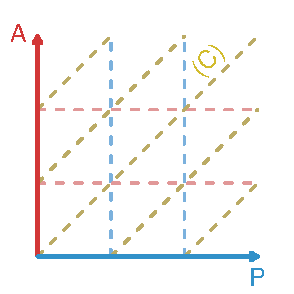
\includegraphics[scale=.5]{AP_rt.pdf}
%  \\
%  %%%% ACp
%  $$\begin{aligned}
%    &\text{AC(P)} \\
%    &\text{P = C + A}
%  \end{aligned}$$ &
%  The AC(P) temporal plane is equivalent to the Lexis diagram except birth
%  cohort is given and period is derived rather than the other way around. &
%  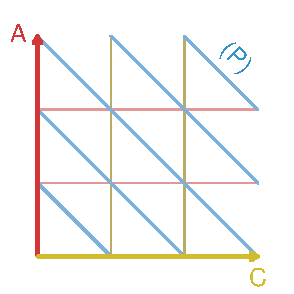
\includegraphics[scale=.5]{AC_rt.pdf} 
%   \\
%  %%%% CPa
%  $$\begin{aligned}
%    &\text{CP(A)} \\
%    &\text{A = P -- C}
%  \end{aligned}$$ &
%  The CP(A) temporal plane is equivalent to the Lexis diagram except birth
%  cohorts are given and age is derived rather than the other way around. &
%  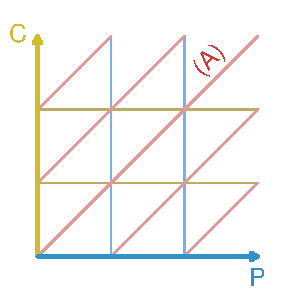
\includegraphics[scale=.5]{CP_rt.pdf}  
%  \\
%  \midrule
%  %%%%%%%%%%%%%%%%%%%%%%%%%%%%%%%%%%%%%%%%%%%%%%%%%%%%%%%%%%%%%%%%%%%%%%%%%%%%%
%  \multicolumn{3}{c}{\textsc{Variants of TPD}} \\
%  \midrule
%  %%%% TPd
%  $$\begin{aligned}
%    &\text{TP(D)} \\
%    &\text{D = P + T}
%  \end{aligned}$$ &
%  Helen had 30 years of life left (T) in 1971 (P) and therefore belonged to the 2001 death cohort (D) &
%  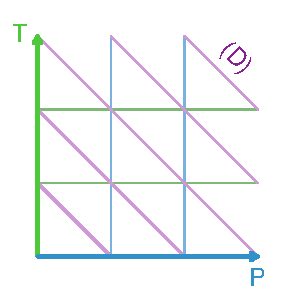
\includegraphics[scale=.5]{TP_rt.pdf}  
%   \\
%  %%%% PDt
%  $$\begin{aligned}
%    &\text{PD(T)} \\
%    &\text{T = D -- P}
%  \end{aligned}$$ &
%  Mindel died in 1973 (D). In 1953 (P) she had 20 years left to live (T). &
%  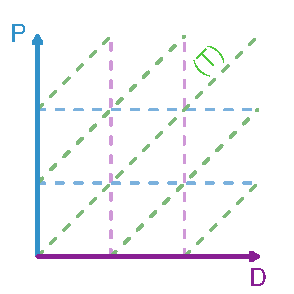
\includegraphics[scale=.5]{PD_rt.pdf} 
%   \\
%  %%%% TDp
%  $$\begin{aligned}
%    &\text{TD(P)} \\
%    &\text{P = D -- T}
%  \end{aligned}$$ &
%  Irene died in 1974 (D). When she had 30 remaining years of life (T) the year must have been 1944 (P). &
%  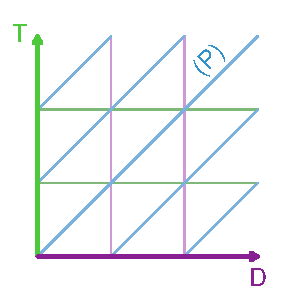
\includegraphics[scale=.5]{TD_rt.pdf}   
%  \\
%  \midrule
%  %%%%%%%%%%%%%%%%%%%%%%%%%%%%%%%%%%%%%%%%%%%%%%%%%%%%%%%%%%%%%%%%%%%%%%%%%%%%%
%  \multicolumn{3}{c}{\textsc{Variants of TAL}} \\
%  \midrule
%  %%%% TAl
%  $$\begin{aligned}
%    &\text{TA(L)} \\
%    &\text{L = T + A}
%  \end{aligned}$$ &
%  The time already lived and the time still left sum up to the total lifespan. &
%  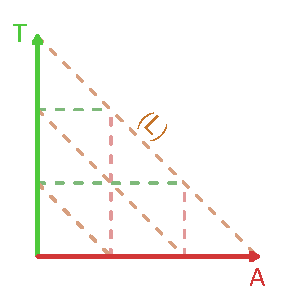
\includegraphics[scale=.5]{TA_rt.pdf}   
%  \\
%  %%%% TLa
%  $$\begin{aligned}
%    &\text{TL(A)} \\
%    &\text{A = L -- T}
%  \end{aligned}$$ &
%  Helen lived to the age of 86 (L). When she had 20 years left (T) she must have been 66 (A). &
%  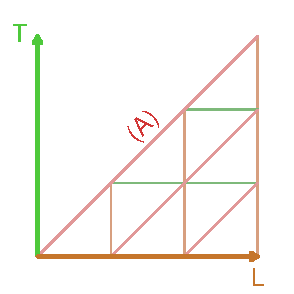
\includegraphics[scale=.5]{TL_rt.pdf}   
% \\
%  %%%% ALt
%  $$\begin{aligned}
%    &\text{AL(T)} \\
%    &\text{T = A -- L}
%  \end{aligned}$$ &
%  Tim is 34 years old (A) and will live to the age of 96 (L), leaving him 62 years (T) to settle affairs. &
%  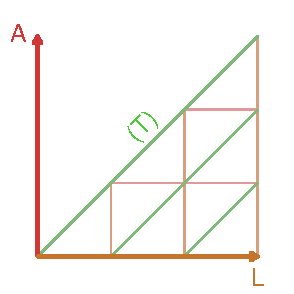
\includegraphics[scale=.5]{AL_rt.pdf} 
%  \\
%  \midrule
%  %%%%%%%%%%%%%%%%%%%%%%%%%%%%%%%%%%%%%%%%%%%%%%%%%%%%%%%%%%%%%%%%%%%%%%%%%%%%%
%  \multicolumn{3}{c}{\textsc{Variants of LCD}} \\
%  \midrule
%  %%%% LCd
%  $$\begin{aligned}
%    &\text{LC(D)} \\
%    &\text{D = C + L}
%  \end{aligned}$$ &
%  \`{A}ngels was born in 1940 (C) and she lived to be 64 (L), implying an
%  untimely death in 2004 (D) &
%  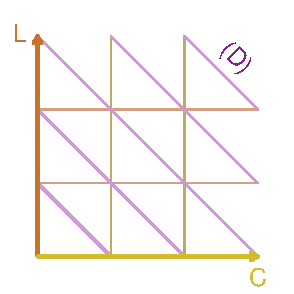
\includegraphics[scale=.5]{LC_rt.pdf}   
%  \\
%  %%%% CDl
%  $$\begin{aligned}
%    &\text{CD(L)} \\
%    &\text{L = D -- C}
%  \end{aligned}$$ &
%  Pascal was born in 1893 (C) and died in 1964 (D), implying a lifespan of 71 (L), or so. &
%  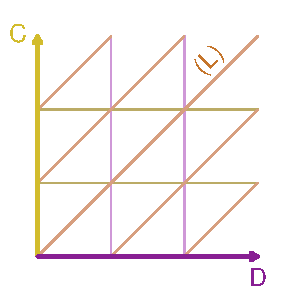
\includegraphics[scale=.5]{CD_rt.pdf} 
%  \\
%  %%%% LDc
%  $$\begin{aligned}
%    &\text{LD(C)} \\
%    &\text{C = D -- L}
%  \end{aligned}$$ &
%  Margaret died in Dec., 1995 (D) with a completed lifespan of 96 (L), putting her birth year in 1900 (C). &
%  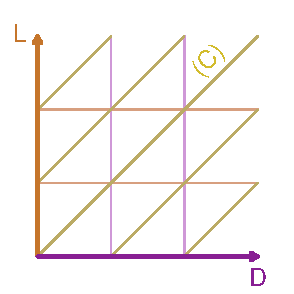
\includegraphics[scale=.5]{LD_rt.pdf}  
%  \\
%  \midrule
%  %%%%%%%%%%%%%%%%%%%%%%%%%%%%%%%%%%%%%%%%%%%%%%%%%%%%%%%%%%%%%%%%%%%%%%%%%%%%%
%  \multicolumn{3}{c}{\textsc{The Uninformative Dyads}} \\
%  \midrule
%  %%%% LP
%  LP(-) &
%  The LP plane is \emph{non-informative}. No additional measures can be derived knowing just lifespan and period. &
%  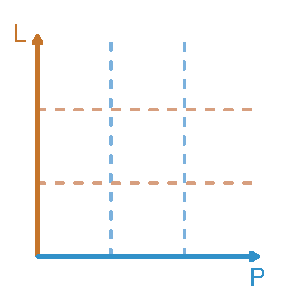
\includegraphics[scale=.5]{LP_rt.pdf} 
%  \\
%  %%%% CT
%  CT(-) &
%  The CT plane is \emph{non-informative}. No additional measures can be derived
%  knowing just birth cohort and thanatological age. &
%  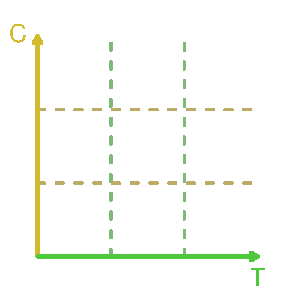
\includegraphics[scale=.5]{CT_rt.pdf} \\
%  %%%% AD
%  AD(-) &
%  The AD plane is \emph{non-informative}. No additional measures can be derived
%  knowing just death cohort and age. &
%  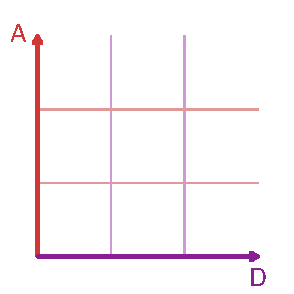
\includegraphics[scale=.5]{AD_rt.pdf} 
%\\
%  \bottomrule
%\end{longtable}

Most of what we know about how rates change over age and time comes
from the very first juxtaposition in Table~2, AP(C). While
CP(A) and AC(P) are statistically redundant when exact times are used, they
are not fully redundant if based on discrete double-classification of data, as
often provided in aggregated official statistics. Double classified data are
found on the APC diagram in the shape of squares (AP), horizontal parallelograms
(AC) and vertical parallelograms (CP), and
these are commonly used to compute different kinds of demographic
rates and probabilities \citep[p.~63]{caselli2005demography}. The other dyadic
juxtapositions (involving the measures T, D, or L) can be considered as either
rare or novel ways of structuring or viewing temporal variation in demography,
and these imply new families of rates and probabilities.

\subsection{The triad identities}
\label{sec:triads}
There are $20=\binom{6}{3}$ ways to choose three different time indices out of
six, of which four form a triad identity: APC, TPD, TAL, and LCD.
Given the three time measures from any of the
triad identities, one can derive no further time measures. If one selects three
random time indices that do not form any of these four triad identities
($20-4=16$ possibilities), this property does not hold. For instance, in the
triad APT, age and period are not sufficient to determine thanatological age.
Given the triad APT one can however derive the remaining three time
measures.

Triad identities are more meaningful than uninformative dyads. This
is so even in the absence of data, due to the underlying relationship between
measures. Each of the triad identities can accommodate some version of a
lifeline, for instance. In the following, we therefore lay out the four primary
diagrams that belong to the triad identities. The question of which diagram
mapping is relevant to a given demographic phenomena is a function of
patterns in the data. The best diagram is the one that captures all meaningful
variation in the data. If APC highlights meaningful variation in a phenomenon,
then its representation as such is useful, and the same holds for the other
identities.

\subsubsection{APC: Chronological age, period, and birth cohort}
\label{sec:apc}
\FloatBarrier
The Lexis diagram has long been used in demography as a conceptual
tool for structuring data, observations, and rate estimation, as inspiration for work
on statistical identification, and as the coordinate basis of contemporary
Lexis-surfaces. Since the Lexis diagram could have been named for others
\citep{keiding2011age, vandeschrick2001lexis}, and since we compare with other
temporal configurations, we refer to it as the APC diagram. 

[ Figure 1 about here ]
%\begin{figure}[h!] 
%\caption{An APC diagram with six lifelines.}
%\label{fig:APC}
%\centering
%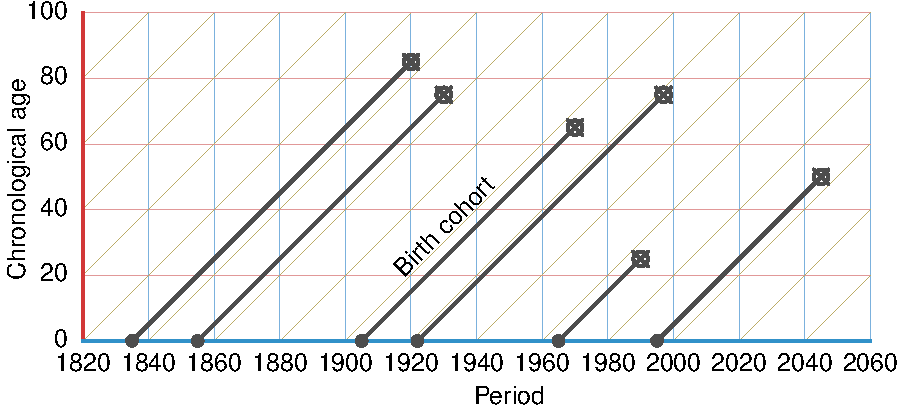
\includegraphics[scale=0.8]{Fig1.pdf}
%\end{figure}

The APC diagram in Fig.~1 represents years lived on the $y$
axis, calendar years on the $x$ axis, and birth cohorts as the right-ascending
diagonals. This is the most common of several possible configurations
of the APC dimensions. Individual lifelines (black) are aligned in the birth
cohort direction, starting with birth (filled circle) at chronological age zero, and death
(circled x). Any APC surface can be interpreted along each of these
three dimensions of temporal structure. 

\FloatBarrier
\subsubsection{TPD: Thanatological age, period, and death cohort}
\label{sec:tpd}
The TPD diagram is best imagined as the inverse of the APC diagram. One may take
the same individuals represented in Fig.~1 and group them by death cohorts (D) instead
of birth cohorts (C). Lifelines then descend such that all
endpoints align to thanatological age 0, creating the diagram in
Fig.~2 in which individuals dying at different ages but in the same time period are grouped together.
To our knowledge, the TPD diagram has only appeared once in the literature, as
a didactic aid in a proof of symmetry between chronological and thanatological
age structure in discrete stationary populations \citep{villavicencioRiffeSymmetires2016}. TPD
diagrams may also be useful to arrange events or durations that are logically
aligned (or may only be aligned) by time of termination. It may be reasonable to
align on termination in cases where this brings preceding patterns of
variation into focus.

[ Figure 2 about here ]
%\begin{figure}[h!] 
%\caption{A TPD diagram with six lifelines.}
%\label{fig:TPD}
%\centering
%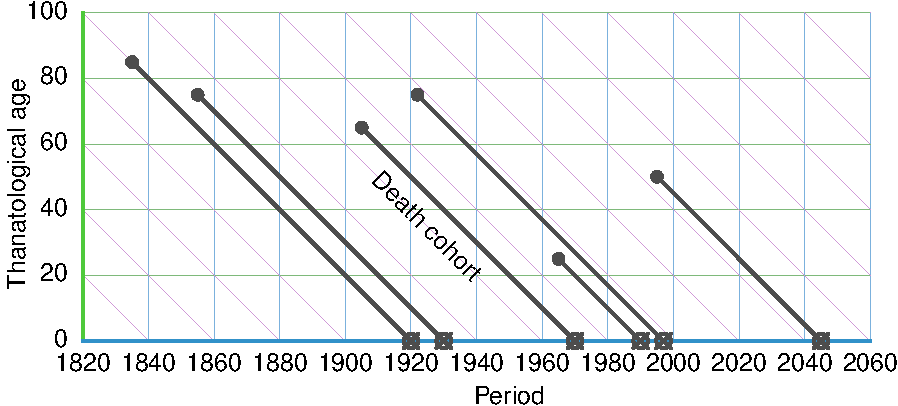
\includegraphics[scale=0.8]{Fig2.pdf}
%\end{figure} 

There are several examples of analysis of this kind of data, usually stemming
from a lack of information on chronological age. This is the case, for instance,
in biodemographic studies in which wild animals with unknown ages are captured
and then followed-up until death \citep{muller2004demographic,
muller2007survival}. Other examples are human historical databases, which
usually lack information about births, but individuals can be traced from a
particular event until death. This is the case in the Barcelona Historical
Marriage Database, which collects information about marriage licenses of
Barcelona (Spain) from the mid-fifteenth century until the early twentieth
century. In this database, ages are unknown, but individuals are first
identified in their marriage record and an estimation of the times of death is
plausible \citep{villavicencio2015reconstructing}. We speculate that TPD
diagrams could also be used in biomedical studies for the representation of
lifelines preceding deaths from infectious or acquired conditions, when the time
of infection or acquisition remains unknown, an issue which has received
attention in the statistical literature \citep[see e.g.][]{chan2010backward}.

\FloatBarrier
\subsubsection{TAL: Thanatological age, chronological age, and
lifespan}
\label{sec:tal}
\FloatBarrier  
TAL is an appropriate diagram to examine processes that vary over the
life course.
More precisely, the TAL plane can highlight variation that is related to time
since birth, time until death, length of life, and their combinations. These
key aspects of demographic time are compressed to chronological age only in the
APC perspective, which can blend out meaningful variation. Since the life course
belongs to the cohort perspective, it is best to think of the TAL plane as belonging to some particular birth cohort. Alternatively, a TAL triangle may be taken as a cross-section through the period dimension, a sort of synthetic TAL plane.

To our knowledge, the TAL diagram has only appeared once in the literature, in an exploration and classification of late-life health
conditions \citep{riffe2016ttd}. There are however instances of statistical
designs adapted to this coordinate plane \citep[see e.g.,][]{dempsey2016, Jewell2016}. The TAL diagram in Fig.~3 contains no indication of
period or cohorts, as calendar time is blended out in this diagram.
The lifelines depicted are identical to those shown in APC Fig.~1
and TPD Fig.~2. The TAL diagram is useful for characterizing patterns of prevalence of health conditions. We speculate
that data structured and aligned in this way may yield hitherto undescribed
patterns in other contexts, e.g. measurements on mother and fetus over the
course of a pregnancy may vary by age of gestation, time until parturition, or
total length of the pregnancy; growth and reproduction patterns over age may be conditioned on the life-span of an organism.

[ Figure 3 about here ]
%\begin{figure}[h!] 
%\caption{A TAL diagram with six lifelines. Since two of the six lifelines are
% of equal length (75), they are overlapped in this figure and appear to be five.}
%\label{fig:TAL}
%\centering
%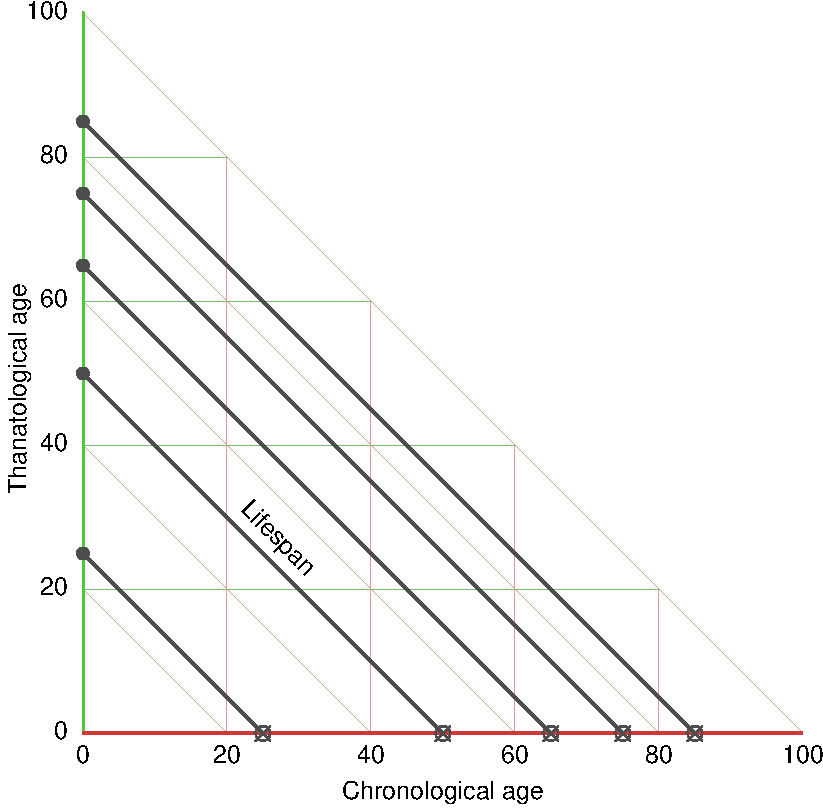
\includegraphics[scale=0.7]{Fig3.pdf}
%\end{figure} 

\FloatBarrier
\subsubsection{LCD: Lifespan, birth cohort, and death cohort}
\label{sec:lcd}
\FloatBarrier

The LCD diagram completes our set of identities. It is based on the relationship
between lifespan, birth cohort, and death cohort. In
Fig.~4, lifespans are indexed by the $y$-axis, while birth cohorts are indexed by the $x$-axis, and death cohorts
are found in descending diagonals. To structure data on these three
time measures implies excluding time-varying information over the life course.
An individual
only ever has one lifespan, one birth cohort, and one death cohort, such that
the LCD coordinates of an individual are constant throughout life.
The LCD plane is therefore orthogonal to lifelines, and individuals are located
with points, rather than life segments.
In Fig.~4, the same six individuals from previous diagram figures are represented with crossed circles.

[ Figure 4 about here ]
%\begin{figure}[h!] 
%\caption{An LCD diagram with six lifelines. Since the LCD plane is orthogonal
%to the life course, lifelines are depicted as points.}
%\label{fig:LCD}
%\centering
%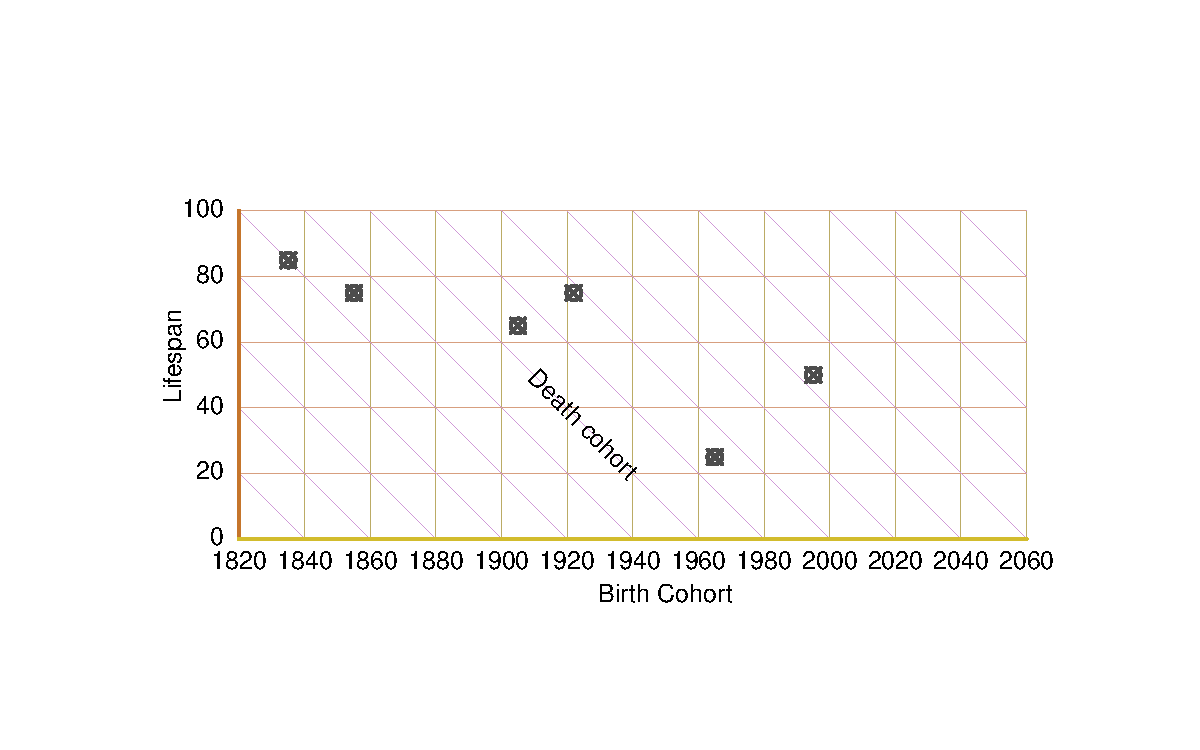
\includegraphics[scale=0.8]{Fig4.pdf}
%\end{figure} 

We recommend this mapping for plotting surfaces of values that are cumulative or
static over the life course, but that may vary over time or by length of life.
Imagine an LCD surface of cumulative life course consumptive surplus or deficit,
or anything else that might vary by lifespan and moment of birth or death, such as children ever born, years of retirement, the
size of trees or other aspects of forestry, populations of buildings in large
cities, and so forth. \citet{lexis1875einleitung} describes an analogous
relationship between marriage cohort, separation cohort, and duration of
marriage.

\FloatBarrier

\section{The relationship between events and durations}
\label{sec:gen}
The four identity-based diagrams discussed in prior sections are likely
straightforward, either because the Lexis diagram is already
familiar to the reader, or because Cartesian representations are widely used.
However, the special relationship between these diagrams is based on a single
hexad identity, which is less straightforward, and its resultant
diagram is best derived from a more general groundwork. In this section we therefore describe a more general
approach to understanding and constructing higher order temporal identities.
This approach is based on a categorization of time measures into events and
durations, and the realization that durations derive from events in calendar
time.

\subsection{A general framework}
\label{sec:framework}

The general relationship between events and durations serves not only to
introduce the full demographic time framework, but also to compare it with
other relatively complicated temporal designs in the literature. Each of the six
time measures that we have treated can be categorized into two basic types:
events and durations. Events include birth (C) and death (D) cohort, as well as period
itself (P). Durations are time differences between pairs of events: chronological age A = P -- C, 
thanatological age T = D -- P, and lifespan L = D -- C. In the following we
describe APC, APCTDL and other time frameworks in terms of vector spaces which, via linear transformation, relate the timing of events with durations between events.

\begin{definition} 
  Let $\boldsymbol{p}=(p_1,\ldots,p_n)^\top\in\mathbf{R}^n$ be a vector of $n$
  events or points in time with $n\geq2$. A corresponding vector of durations $\boldsymbol{d}\in\mathbf{R}^m$ is composed by elements of the form $d_{i,j}=p_j-p_i$ for $i=1,\dots,n-1$, $j=2,\dots,n$ and $j>i$.
  \label{def:1}
\end{definition}

The vector of events $\boldsymbol{p}$ can be ordered in an arbitrary way as long as the same elements in $\boldsymbol{p}$ correspond to the same type of event for all observations. A consequence of this is that durations may be either
negative or positive depending on the ordering of events over the life course.

\begin{proposition}
  Given a vector of events $\boldsymbol{p}=(p_1,\ldots,p_n)^\top\in\mathbf{R}^n$, the dimension of the corresponding vector of durations $\boldsymbol{d}\in\mathbf{R}^m$ is $m=n(n-1)/2$.
\end{proposition}

\begin{proof}
  By definition, each element of $\boldsymbol{d}$ is formed by two different elements of $\boldsymbol{p}$. Therefore, the length of $\boldsymbol{d}$ is the number of combinations of 2 different elements from a set of size $n$, such that the order of selection does not matter. From combinatorial theory, it is well known that this value is given by the binomial coefficient $\binom{n}{2}=\frac{n!}{2!(n-2)!}=n(n-1)/2$.
\end{proof}

\begin{proposition}
 For any vector of events $\boldsymbol{p}=(p_1,\ldots,p_n)^\top\in\mathbf{R}^n$, there is always a linear transformation $f:\mathbf{R}^n\to\mathbf{R}^m$ that provides a corresponding vector of durations $\boldsymbol{d}\in\mathbf{R}^m$.
 \label{prop:2}
\end{proposition}

\begin{proof}
 The existence of $f$ is a direct consequence of Definition~\ref{def:1}, given that all the elements of $\boldsymbol{d}$ are a linear combination of elements of $\boldsymbol{p}$. 
\end{proof}

\begin{corollary}
 Given $\boldsymbol{p}=(p_1,\ldots,p_n)^\top\in\mathbf{R}^n$, suppose that $\boldsymbol{d}=(p_2-p_1,\dots,p_n-p_1,p_3-p_2,\dots,p_n-p_2,\dots,p_n-p_{n-1})$. Then, the linear transformation $f:\mathbf{R}^n\to\mathbf{R}^m$ that yields $\boldsymbol{d}$ from $\boldsymbol{p}$ is defined by the $m\times n$ matrix
 %
 \begin{align}
  \boldsymbol{X}_{(m\times n)}&= \left(\begin{array}{cccccc}
			  \multicolumn{1}{c:}{-1}			& \multicolumn{5}{c}{}					\\
			  \multicolumn{1}{c:}{\vdots}	 		& \multicolumn{5}{c}{I_{n-1}}	 			\\  
			  \multicolumn{1}{c:}{-1}			& \multicolumn{5}{c}{}					\\ \hdashline
			  0		& \multicolumn{1}{c:}{-1}	& \multicolumn{4}{c}{}					\\	 
			  \vdots	& \multicolumn{1}{c:}{\vdots}	& \multicolumn{4}{c}{I_{n-2}}  				\\
			  0		& \multicolumn{1}{c:}{-1}	& \multicolumn{4}{c}{}					\\ \hdashline
			  \multicolumn{6}{c}{\cdots}										\\ \hdashline
			  0		& \cdots	& 0		& \multicolumn{1}{c:}{-1}	& 	& 		\\ 
			  0		& \cdots	& 0		& \multicolumn{1}{c:}{-1}	& \multicolumn{2}{c}{\smash{\raisebox{.5\normalbaselineskip}{$I_2$}}}	\\ \hdashline
			  0		& \multicolumn{2}{c}{\cdots}	& 0				& -1	& 1		\\
			\end{array}\right)
  \label{eq:matrix}\ ,
 \end{align}
  %
 such that $\boldsymbol{d}=\boldsymbol{X}\times\boldsymbol{p}$, and where $I_k$ denotes the $k\times k$ identity matrix.
\end{corollary}

These results imply that given an arbitrary set of $n\geq2$ points in time, it
is always possible to calculate the durations between any pair of these points. However, note that matrix $\boldsymbol{X}$ in \eqref{eq:matrix} yields a vector of durations $\boldsymbol{d}\in\mathbf{R}^m$ whose elements are sorted in an arbitrary way. The following statement may be relevant in this regard.

\begin{proposition}
 Given a vector of events $\boldsymbol{p}=(p_1,\ldots,p_n)^\top\in\mathbf{R}^n$, the corresponding vector of durations $\boldsymbol{d}\in\mathbf{R}^m$ is unique, irrespective of the sorting of its elements.
\end{proposition}

\begin{proof}
 Let's suppose that $\boldsymbol{d^1}$ and $\boldsymbol{d^2}$ are two different
 vectors of durations corresponding to the same vector of events
 $\boldsymbol{p}\in\mathbf{R}^n$. Provided that $\boldsymbol{d^1}$ and
 $\boldsymbol{d^2}$ are finite and, by definition, both have dimension $m$ and are formed by the same combinations of elements of $\boldsymbol{p}$, it will always be possible to re-arrange the elements of $\boldsymbol{d^2}$ in the same order as $\boldsymbol{d^1}$ such that $\boldsymbol{d^1}=\boldsymbol{d^2}$.
\end{proof}

This last proposition allows considering $\boldsymbol{X}$ as the matrix defining
the linear transformation between points and durations. Given a vector
$\boldsymbol{p}$ and the corresponding
$\boldsymbol{d}=\boldsymbol{X}\times\boldsymbol{p}$, any differently sorted
vector of durations would be obtained by swapping the rows of $\boldsymbol{X}$.
Further, note that $\boldsymbol{X}$ does not have an inverse matrix, and
therefore there is no linear transformation from durations to events. This is
intuitively straightforward if one thinks that two vectors of events can yield
the same vector of durations. In other words, a particular vector of durations
can come from infinite different vectors of points in time. For instance, using
$\boldsymbol{X}$, the vectors of events $\boldsymbol{p^1}=(1,2,3)$ and
$\boldsymbol{p^2}=(2,3,4)$ both yield $\boldsymbol{d}=(1,2,1)$. With respect to
the six time measures discussed here, note that the events CPD yield TAL, but TAL does not yield CPD.

The relationship between events and durations can be
systematically represented in a series of timelines and graphs that may better
guide intuition.
The joint relationship between events and durations is more explicit and more
compact in a graph representation. As introduced in the following definition, the total number of time measures implied by a set of $n$ events and the corresponding durations is 
$n+m=n+n(n-1)/2=n(n+1)/2$. 

\begin{definition}
Given a vector of events $\boldsymbol{p}=(p_1,\ldots,p_n)^\top\in\mathbf{R}^n$, $n\geq2$, and the corresponding vector of durations $\boldsymbol{d}\in\mathbf{R}^m$, we define the graph of time measures
 $\boldsymbol{G}$ as the graph with $n+m=n+n(n+1)/2$ edges labelled by
 $(\boldsymbol{p},\boldsymbol{d})\in\mathbf{R}^{n(n+1)/2}$ such that the relationships in Definition~\ref{def:1} are preserved.
 \label{def:2}
\end{definition}

Table~3 displays a timeline and a graph for two, three, and four event sets. The central column shows timelines, a familiar linear representation of time, with events
marked with red ticks labelled with $p_1 \ldots p_n$. Durations span
each of the $m$ possible event dyads and are drawn below
the main timeline as curly braces labelled with $d_{1,2} \ldots d_{n-1,n}$. The right
column of Table~3 draws the corresponding graph with a total of $n+1$ vertices and $n+m=n(n+1)/2$ edges
for the elements of both $\boldsymbol{p}$ and $\boldsymbol{d}$. All
events of $\boldsymbol{p}$ connect to a single vertex, and event edges are
indicated in red with red-circled labels. In this rendering, each triangle formed by three
mutually connecting edges represents a triad identity. The top row $n=2$
consists in a single identity. Three and four events imply a total of four and
ten triad identities, respectively, and in general a given higher order identity
will yield $\binom{n+1}{3}$ triad identities.
We call this a temporal plane graph because the triangle resulting from any given triad sub-identity can be extended over
all valid values of its time measures to form a temporal plane, as of the
diagrams in Sect.~\ref{sec:triads}. The dimensionality of the extended diagram of a given identity follows from the
number of events from which the identity is derived: $n=2$ produces a
two-dimensional diagram, $n=3$ produces a 3-dimensional diagram, and so forth.

%\newcolumntype{S}{ >{\centering\arraybackslash} m{2cm} }
%\newcolumntype{D}{ >{\centering\arraybackslash} m{5.4cm} }
%\newcolumntype{E}{ >{\centering\arraybackslash} m{3.7cm} }

[ Table 3 about here ]

%\begin{table}[ht]
%\centering
%\caption{Event-duration timeline and graph for two, three, and four event
% sequences.}
%\label{tab:timelines}
%\makebox[\linewidth][c]{
%\begin{tabular}{S D E}
%nr. events  & timeline & graph \\
%& &\\
%  $n = 2 $ & \Tl{2} & \Ed{2} \\
%  $n = 3 $ & \Tl{3} & \Ed{3} \\
%  $n = 4 $ & \Tl{4} & \Ed{4}
%\end{tabular}
%}
%\end{table}

\begin{definition} 
  We define $P\subseteq\mathbf{R}^n$ as the vector-space (event-space) spanning all possible values vector $\boldsymbol{p}$ may take, and $D\subseteq\mathbf{R}^m$ as the vector space spanning all possible instances of the duration vector $\boldsymbol{d}$. 
  % (FV removed) Let the indices of the bases of $P$ and $D$ correspond to the
  % indices of elements of $\boldsymbol{p}$ and $\boldsymbol{d}$.
  \label{def:1b}
\end{definition}

Just like the APC diagram allows for \emph{all possible} combinations of period,
cohort and age we may consider the vector space $P$ spanning all possible
instances of $\boldsymbol{p}$. The calculation of durations between events as
described in Proposition~\ref{prop:2} can then be understood as a linear
transformation from a vector space $P$ whose bases represent events to a
duration vector space $D$ whose bases represent durations.

\FloatBarrier
\subsection{Examples}
\label{sec:examples}
The following examples show how different demographic time frameworks can all be expressed as instances of the event-duration vector space defined above.

\paragraph{Example 1: The Lexis surface}

Let $\boldsymbol{p}$ have two elements, as in the first row of
Table~3. Then $\boldsymbol{d}$ consists of just one element, defined as

\begin{equation}
d_{1,2} = p_2 - p_1   \quad\quad.
\end{equation}
%
Interpreting $d_{1,2}$ as \emph{age}, $p_2$ as \emph{period}, and $p_1$ as
\emph{birth cohort} yields the APC identity. The standard Lexis surface is
constructed via a change of basis from the event-space $P$, featuring basis vectors $(p_1,
p_2)$, to the event-duration space $M$, featuring basis vectors ($p_2, d_{1,2}$).

\paragraph{Example 2: Lexis' marriage identity}

Along with his well known 2-dimensional diagram \citet{lexis1875einleitung} also
described a 3-dimensional extension applied to the marriage and
separation processes, reproduced in \citet{keiding2006event}. Let $\boldsymbol{p}$ have three elements, as in the second row of
Table~3. Then $\boldsymbol{d}$ is defined as

\begin{equation}
\label{eq:p3}
\begin{matrix}
d_{1,2} = p_2 - p_1\\
d_{1,3} = p_3 - p_1\\
d_{2,3} = p_3 - p_2
\end{matrix} \quad\quad.
\end{equation}
%
Interpreting $p_1$ as \textit{birth cohort}, $p_2$ as \textit{marriage cohort} and $p_3$ as
\textit{separation cohort} yields the durations $d_{1,2}$ as \textit{age at
marriage}, $d_{1,3}$ as \textit{age at separation}, and $d_{2,3}$ as
\textit{duration of marriage}. Lexis' ``marriage space'' $M$ is reconstructed by
a change of basis from $P\subseteq\mathbf{R}^3\to M\subseteq\mathbf{R}^3$, with
the new orthogonal basis formed by $(p_1, d_{1,2}, d_{2,3})$.

\paragraph{Example 3: Adding death cohort to the Lexis surface}

As in Example 2 we start with a three element vector
$\boldsymbol{p}$ yielding the very same identities as in Eq.~\eqref{eq:p3} and the second row of Table~3, but with different interpretations.
Interpreting $p_1$ as \textit{birth cohort}, $p_2$ as \textit{period} and $p_3$
as \textit{death cohort} yields the durations $d_{1,2}$ as \textit{chronological
age}, $d_{1,3}$ as \textit{lifespan}, and $d_{2,3}$ as \textit{time to death}.
This vector space contains the Lexis surface as a sub-space, as well as the other planes presented in Sect.~\ref{sec:triads}. We return to this identity
in the following sections.

\paragraph{Example 4: Brinks' Illness-Death model}

\citet{brinks2014lexis} describe an illness-death process atop the Lexis
surface, and with diagnosis and death as additional events, for a total of four
events. Let $\boldsymbol{p}$ have four elements, as in the third row of
Table~3. Then $\boldsymbol{d}$ is defined as:

\begin{equation}
\label{eq:p4}
\begin{matrix}
d_{1,2} = p_2 - p_1\\
d_{1,3} = p_3 - p_1\\
d_{2,3} = p_3 - p_2\\
d_{1,4} = p_4 - p_1\\
d_{2,4} = p_4 - p_2\\
d_{3,4} = p_4 - p_3
\end{matrix} \quad\quad.
\end{equation}

Interpreting $p_1$ as \textit{birth cohort}, $p_2$ as \textit{period}, $p_3$ as
\textit{time at diagnosis}, and $p_4$ as \textit{death cohort} yields the following composition
of $\boldsymbol{d}$: $d_{1,2}$ is \textit{chronological age}, $d_{1,3}$ is
\textit{age at diagnosis}, $d_{1,4}$ is \textit{lifespan}, $d_{2,3}$ is
\textit{time to/since diagnosis},\footnote{For points
in time past the time at diagnosis $d_{2,3}$ becomes negative and can be
interpreted as time since diagnosis.} $d_{2,4}$ is \textit{time to
death}, and $d_{3,4}$ is duration of illness (an irreversible state).

Unlike the other examples, the actual vector-space of demographic
time shown in \citet{brinks2014lexis} Fig.~2 only identifies a
\emph{subset} of the times-measures implied by the model of the
authors, namely age ($y$-axis), period ($x$-axis), birth cohort (implied by a
linear combination of age and period) and duration of disease ($z$ axis).
Although lifelines in this depiction only begin to ascend into the disease
duration axis at the time of disease diagnosis, this event time measure is not
ascribed to an axis per se or implied by the other axes, and no further time
scales can be derived from the three axes drawn.
Instead, a few additional events and durations (death cohort, timing of
diagnosis and duration of disease) are introduced as \emph{markings} within the three
dimensional vector space, just as one would mark \emph{specific} life-lines on
a Lexis-diagram without accounting for \emph{all possible} life-lines.
Instead, the four-dimensional vector-space can be considered as the larger
setting within which this model operates.


\FloatBarrier
\section{A tetrahedron relates the six demographic time measures}
\label{sec:tetrahedron}
The demographic time framework we present includes three events (period, birth
cohort, and death cohort), and it therefore leads to a graph
based on the second row and third column of Table~3, here
redrawn in Fig.~5 with a slight rearrangement of the
vertices, and edges labelled with the six demographic time measures.

There are a total of four triangles in Fig.~5, one for each
of the triad sub-identities, such that each time measure is an element of two
triad identities. Each of these triangles is the
edge-graph of a face of the tetrahedron, ergo each face of the tetrahedron
represents one of the triad identities. It is reasonably straightforward to
imagine this graph as the wire-frame of a 3-d
tetrahedron --- as the 3-d edge structure of the tetrahedron platonic solid.

[ Figure 5 about here ]
%\begin{figure}[h!]
%\centering
%\caption{Tetrahedral graph of demographic time hexad identity, with edges
%labelled by the six time indices.}
%\label{fig:tet}
%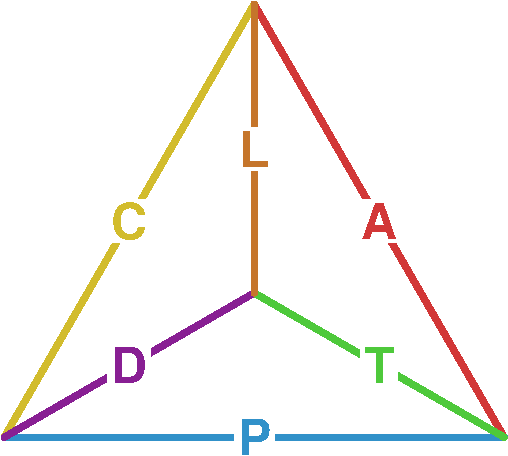
\includegraphics[width=4in]{Fig5.pdf}%
%\end{figure}

For exposition, imagine that the middle vertex of Fig.~5 is the
top (closer to the eye), while the outer edges A, P, and C form the
base of the tetrahedron, forming the much-studied APC identity.
The South face corresponds to the TPD identity,
the Northeast face to the TAL identity, and the
Northwest face to LCD identity. The transformation of this three-event
system to a three dimensional space follows Definition~\ref{def:2}.
It may also suffice to simply imagine that each face of the tetrahedron forms
the basis of a plane, such that the tetrahedron itself defines four planes. These four planes are the four temporal planes that underly
the four diagrams presented in Sects.~\ref{sec:apc} to~\ref{sec:lcd}. A full
diagram of the demographic time identity (or any identity based on three events)
conforms in this way with the geometry of a tetrahedron.


 \section{Diagram of the hexad identity}
 \label{sec:diagram}
 There are different ways to proportion this three dimensional construct,
of which we only present the isotropric mapping.\footnote{To compare,
\citet{lexis1875einleitung} used a Cartesian mapping for his marriage identity,
with right angles between birth cohort, age at marriage, and duration married.}
In an isotropic projection, the tetrahedron is regular, such that all edges are
of the same length, and the units of each of the six represented time measures
are therefore equal. In this case, the four triad identities map to
their respective temporal planes as tessellations of equilateral triangles. When
the plane parallel to each respective face is repeated in equal intervals, we
have an isotropic 3-d space.\footnote{The isotropic space that results from this framework is known in other disciplines with different nomenclatures. In geometry, this structure is called the tetrahedral-octahedral honeycomb, a variety of space-filling tessellation. In
architecture, it is found in the octet truss system. In physics it is called
the isotropic vector matrix. Constructs following this geometry exist in nature,
in other theoretical settings, and in man-made structures.}
Displaying all planes simultaneously creates a very dense and difficult-to-read
diagram. We opt to delineate the space using the intersection of two planes.

Figure~6 gives a view of a demographic
time diagram that corresponds to the hexad identity, where birth-cohort TAL
cross-sectional planes are placed in sequence in a perspective drawing.\footnote{The coordinates used to render Fig.~6 are isotropic.
However, there are no 60$^\circ$ angles in this figure due to the use of
parallax and an indirect viewing angle in this rendering for the sake of
increased legibility.} The most recent TAL plane, for the year 2000, is placed
in the front, whereas past TAL planes are stacked behind it, highlighted in
25-year intervals. The left edge of the frontmost TAL plane is labelled as an
axis for thanatological age, although the same tick marks also serve for
completed lifespan.
The base of this figure is the APC plane, drawn through thanatological age 0.
Each of the TAL planes sits atop a single birth cohort line from the familiar
APC plane that makes up the base of the diagram.

[ Figure 6 about here ]
%\begin{figure}[!h]
%\centering
%\caption[cap]{Diagram of the hexad identity, showing a sequence of TAL
%planes intersecting with a single APC plane at the base.}
%\label{fig:apctTAL}
%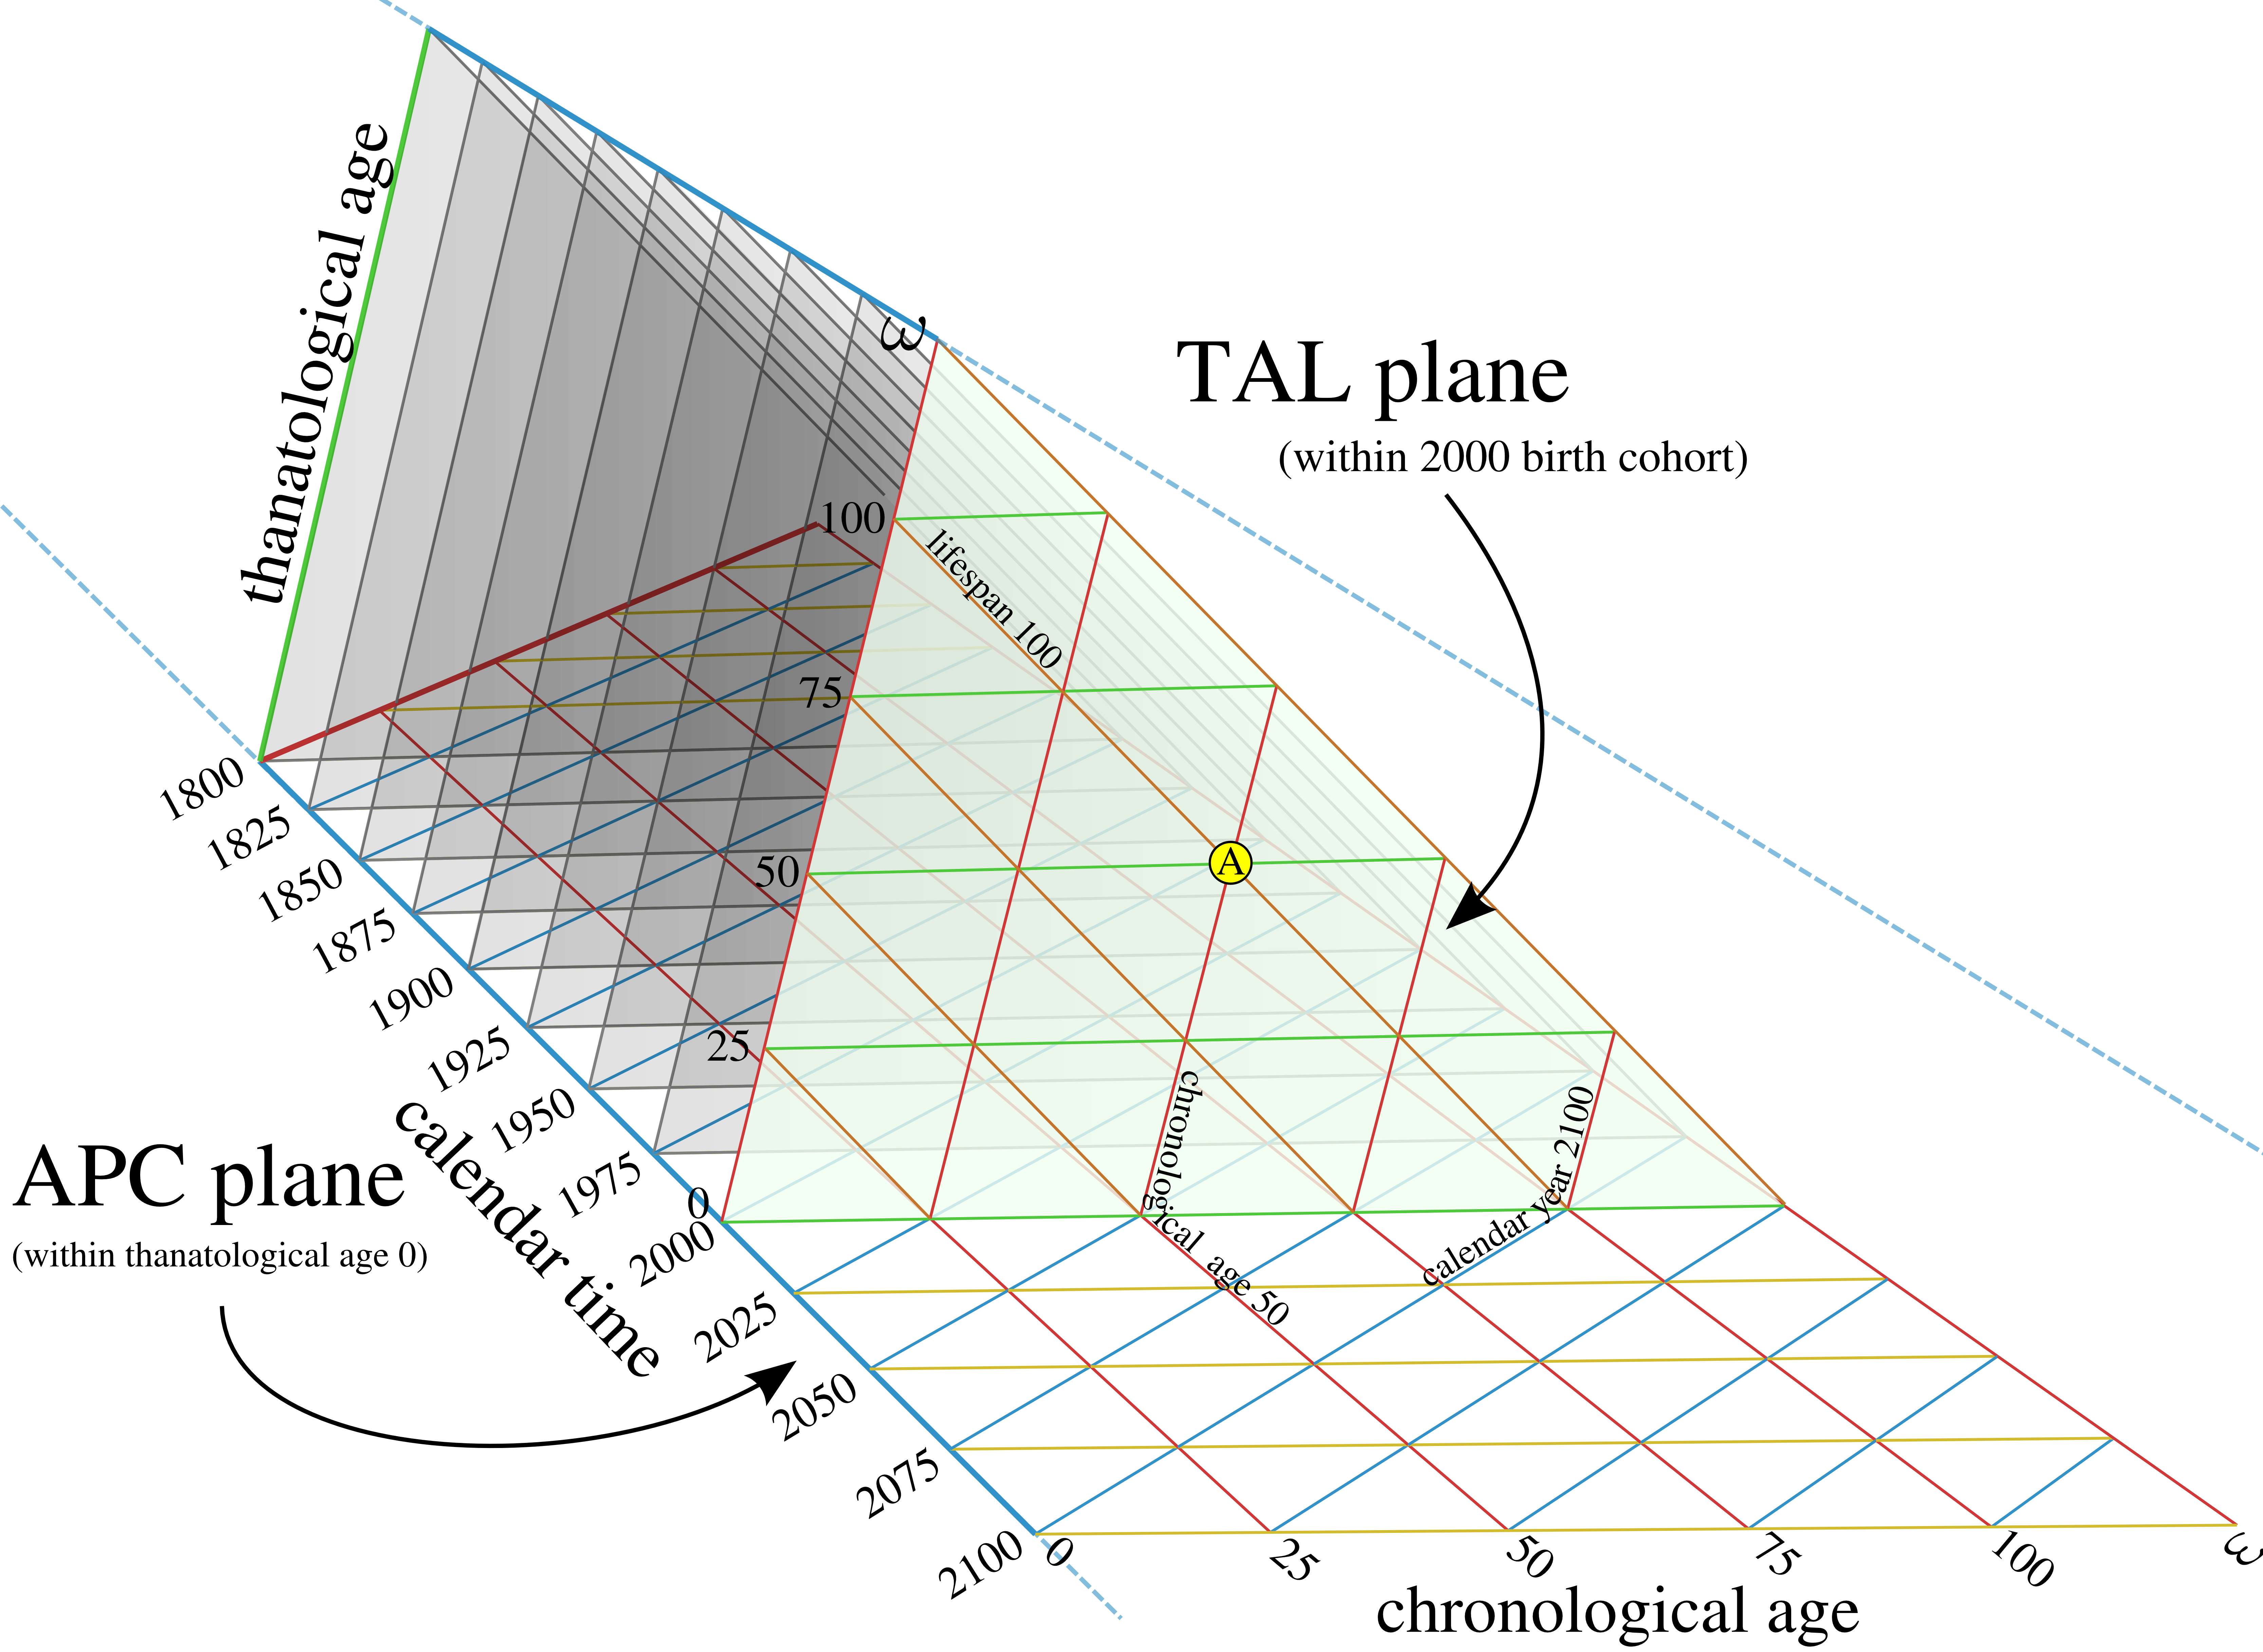
\includegraphics[scale=.5]{Fig6.png} 

% NOTE: Fig6.pdf also available, but note
% transparency needs to be examined for platform and viewer compatibility

%\end{figure}

For example, imagine an infant born in the year 2000. Without further
information, we only know that this infant is located somewhere on the
thanatological age axis (left edge) of the front TAL plane. If this infant is
destined to die in the year 2100, then the vertical position at birth will be at the axis tick for thanatological age 100. This
person's entire life stays on the 100 lifespan line (labelled),
descending over time towards thanatological age 0 at the base. Point A marks the
midpoint in life for this individual, at chronological age 50 (red line, labelled), and
thanatological age 50 (green line). If another APC plane were drawn through thanatological age 50, we would see that point A is in the year 2050. Since all individuals born in the year 2000 complete the same age in the same year, we can
also recuperate the year for point A by following the chronological age 50 line
(red) down to where it meets the blue line for the year 2050. The lifeline
descends downward toward the APC plane for thanatological age 0 at chronological
age 100, meeting the year 2100, which is individual A's death cohort.

The density and location of imaginary lifelines in this diagram, omitting
migration, is purely a function of birth cohort size and survival. For extinct
cohorts all lifelines can be positioned, but for the 2000 birth cohort this is
not yet the case. Most of the front TAL plane is in the future. One may imagine
yet another plane intersecting this space--- the ``present plane'', which is
identical to the period TAL plane for the present moment. To see how this plane
divides the space, imagine that we are in the year 2025, and follow the blue
line in the APC base inward 25 years to where it meets the red line for chronological age 25, and follow the
red line up the front TAL plane. A single plane cuts through the year
2025 and chronological age 25 from the year 2000 birth cohort. This plane
shifts forward or backward in time to meet the present year. In this particular
plane, the coordinates T, L, and D are uncertain. The period TAL plane $\omega$
years in the past is fully identified, ergo, theoretically the lifespan of each
individual in the time of Lexis is knowable. 

Figure~6 could have been drawn with TPD or LCD planes highlighted
as well, but these can still be imagined upon the current rendering. TPD planes
transect this space through any given chronological age, for instance. Imagine a
wall on the left side of the prism, cutting through chronological age 0 (recall
Fig.~2).
In this case, the thanatological age axis is indicated in the very back of the diagram,
calendar time becomes another axis, and death cohort diagonals are not drawn.
TPD planes sequence inward from this first plane, always forming cross-sections
through chronological age. The LCD plane is to be found by rotating the current
prism such that the angle of view is directly orthogonal to lifelines, which
would then appear as points (recall Fig.~4).

The essential property of this perspective diagram is that lifelines
start and end in parallel, desceding downward and forward in time. A real
population of renewing lives, spread over time and over the typical range of
human lifespans, will tend to fill the entirety of the prism depicted in
Fig.~6, and any given point in the prism can be given six
demographic time coordinates, of which three are redundant. A similar 3d
construct could be made for any hexad time-identity, and these are not strictly
limited to event-duration identities based on 3 events.

\FloatBarrier

\section{Application}
\label{sec:app}
The
coordinate system described here may be useful for the visualization of data, to
enable discovery, and to better inform demographic methods. We have not yet
mentioned how such developments might arise in practice. We therefore give a
brief case study to demonstrate the
potential of the present framework, but this is far from an exhaustive
application of its usefulness for other substantive questions, nor is the case study described in complete rigor. Specifically, we reason that
projections or comparisons of prevalence-based healthy life expectancy (HLE) are
in many cases biased in period prevalence-based models unless one takes into account the
thanatological age pattern of prevalence, as well as mortality differences.

There are three steps in our empirical inquiry. The first step is to visualize
variables on health outcomes using the demographic time diagram. The second
step is pattern detection. We assess the primary time measures over which
health outcomes appear to vary.
Under the assumption that these patterns of temporal variation are empirically regular,
we describe a method of standardizing health expectancy calculations
for morbidity conditions whose prevalence is more closely related
to thanatological age.
Finally, we reason that period estimates of health expectancies for certain
health conditions are biased when mortality has been or will-be changing, and
comparisons of HLE between populations with different mortality are also biased.
We conclude that comparisons of health expectancies might be biased in ways not
previously documented.

Let us take the example of self-reported health (SRH). 
 The data come from the RAND version of the US Health and Retirement Study
 \citep{HRSumich,HRS}. Since this survey includes multiple dated observations of
 individuals, as well as information on time of birth and a followup for time of death, we have or
can derive each of the six demographic time measures for each observation.
Further methodological details are given by \citet{riffe2016ttd}. We opt to view
data on TAL surfaces because these allow us to judge the shape of prevalence
over the life course, specifically to show how SRH prevalence variation is
summarized more efficiently as a time-to-death pattern than as an age pattern.

[ Figure 7 about here ]
%\begin{figure}[h!] 
%\caption{Prevalence of males self-reporting poor health by chronological and
%thanatological age, by quinquennial birth cohorts, 1905--1925 (Sources: \citealt{HRSumich, HRS})}
%\label{fig:poorsrh}
%\centering
%\begin{subfigure}{.46\textwidth}
%\centering
%\caption{1905}
%\label{fig:srh1905}
%%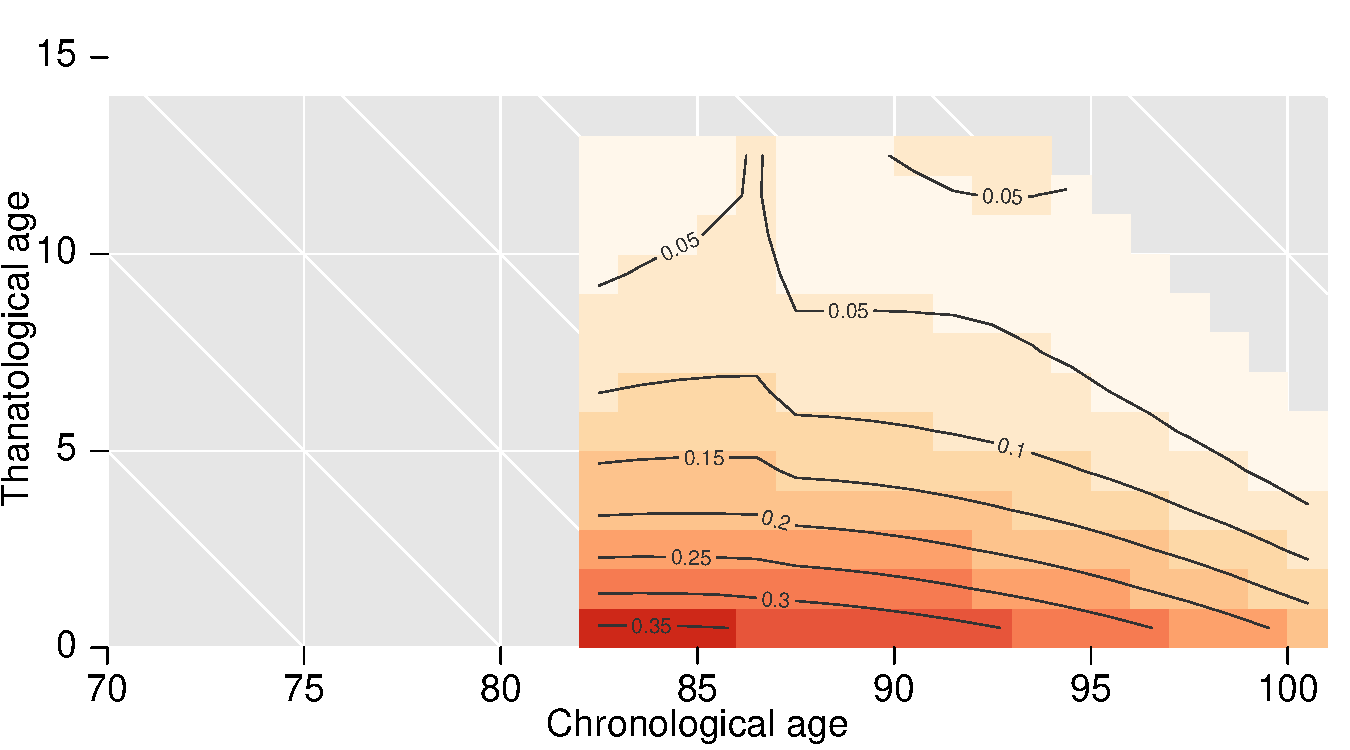
\includegraphics[scale=0.25]{Fig7a.pdf}
%\end{subfigure}
%~
%\begin{subfigure}{.46\textwidth}
%\centering
%\caption{1910}
%\label{fig:srh1910}
%%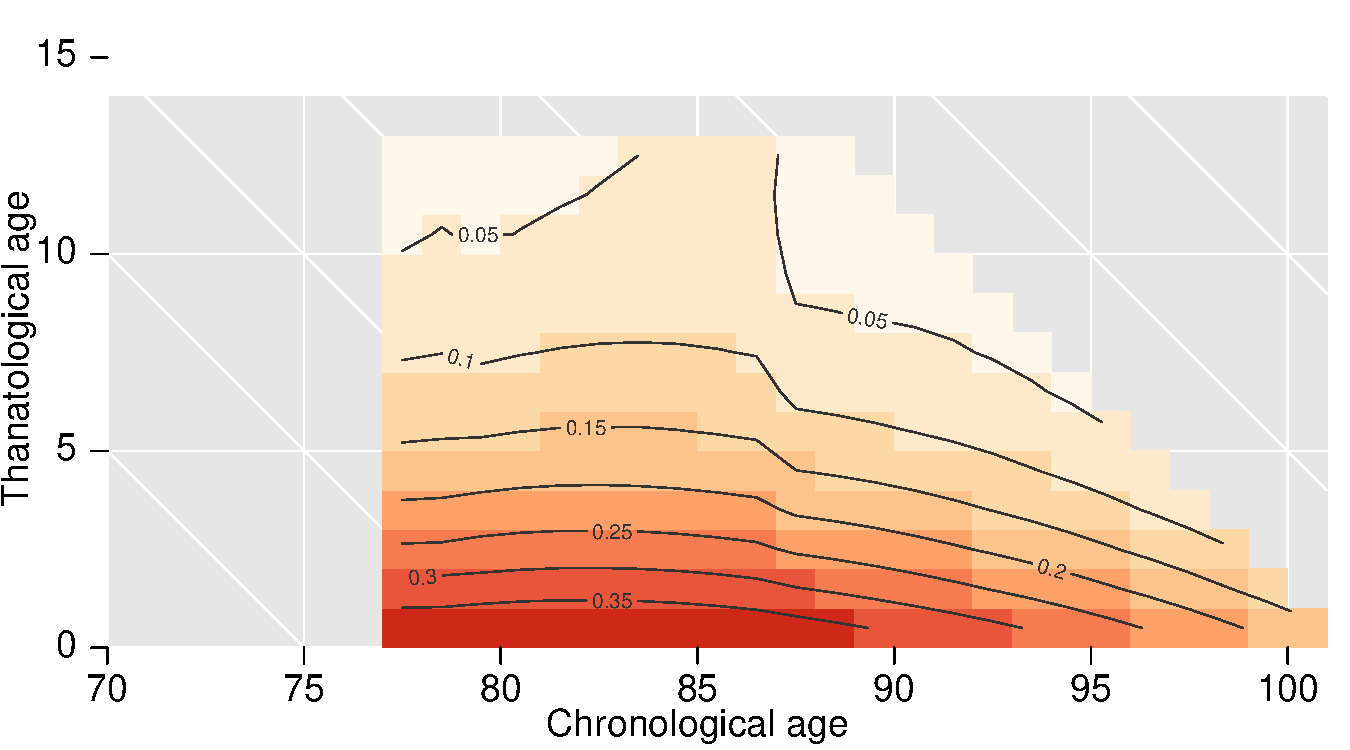
\includegraphics[scale=0.25]{Fig7b.pdf}
%\end{subfigure}
%
%\begin{subfigure}{.46\textwidth}
%\centering
%\caption{1915}
%\label{fig:srh1915}
%%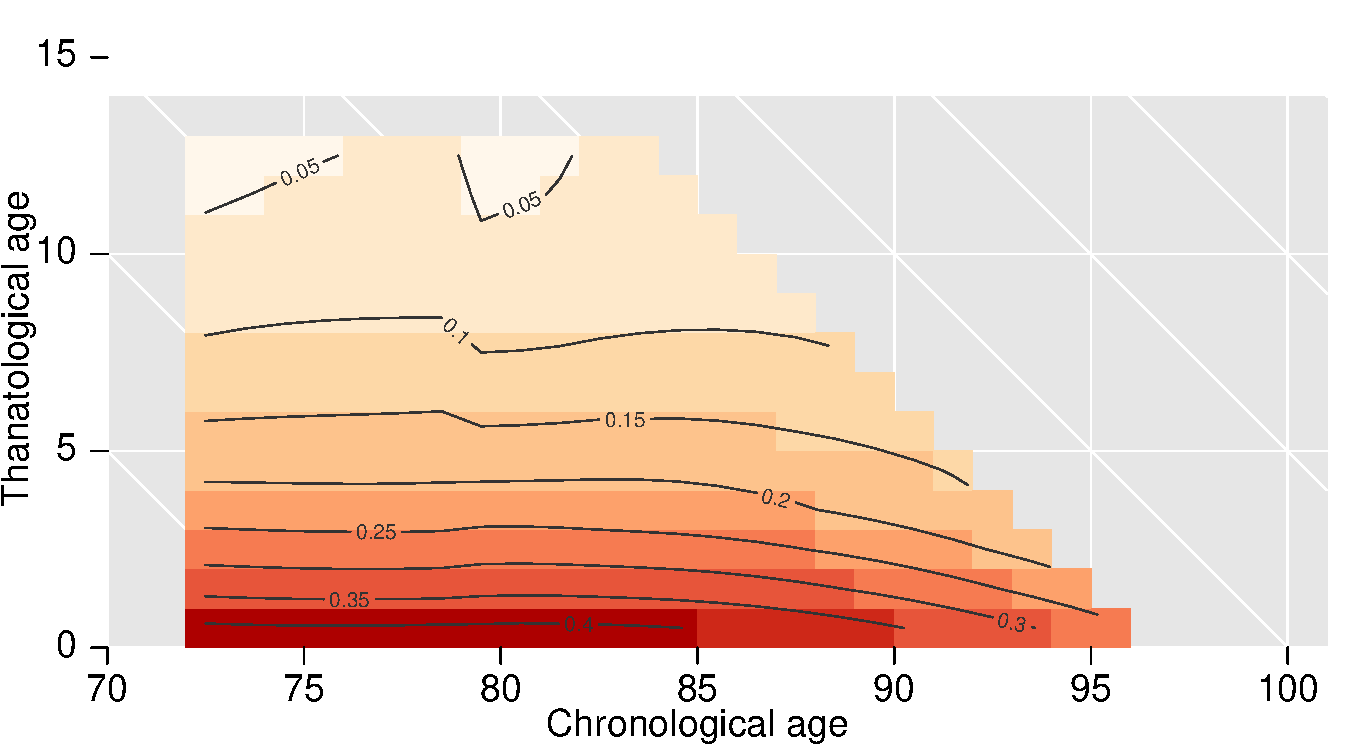
\includegraphics[scale=0.25]{Fig7c.pdf}
%\end{subfigure}
%~
%\begin{subfigure}{.46\textwidth}
%\centering
%\caption{1920}
%\label{fig:srh1920}
%%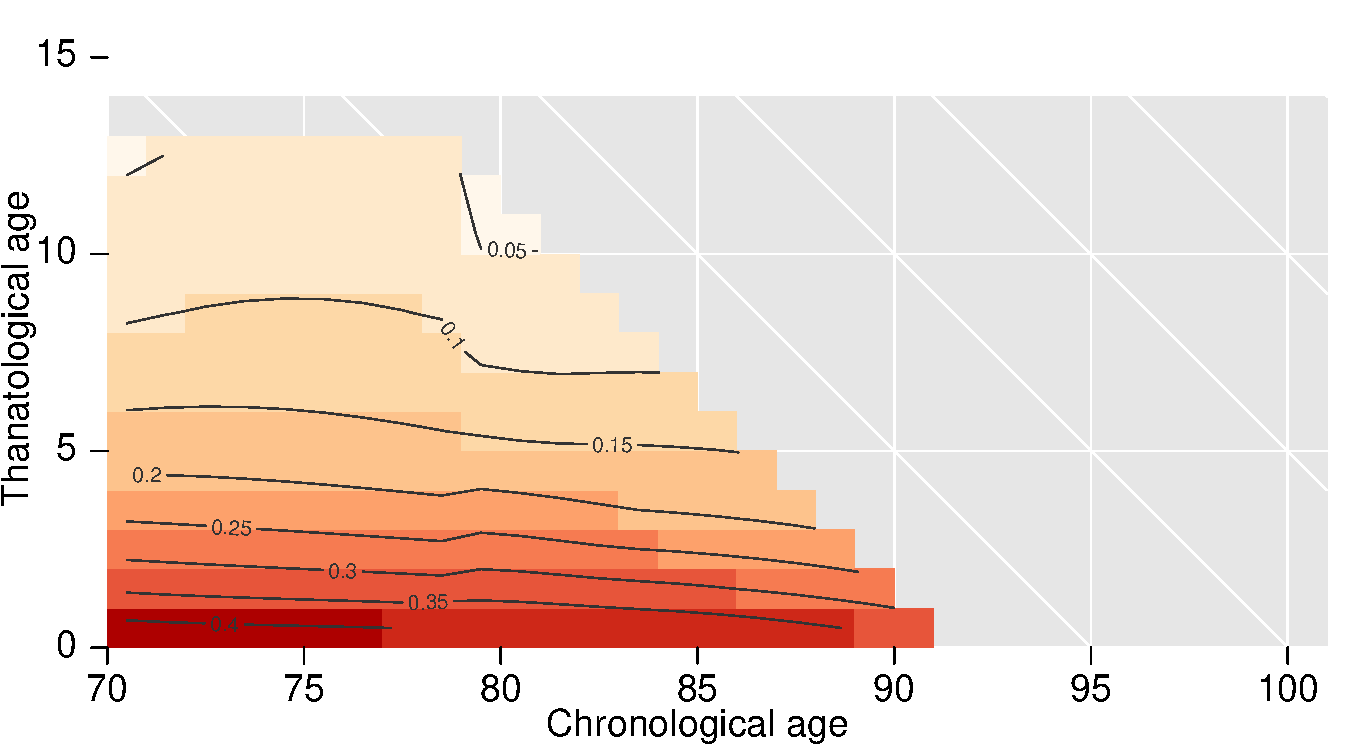
\includegraphics[scale=0.25]{Fig7d.pdf}
%\end{subfigure}
%
%\begin{subfigure}{.46\textwidth}
%\centering
%\caption{1925}
%\label{fig:srh1925}
%%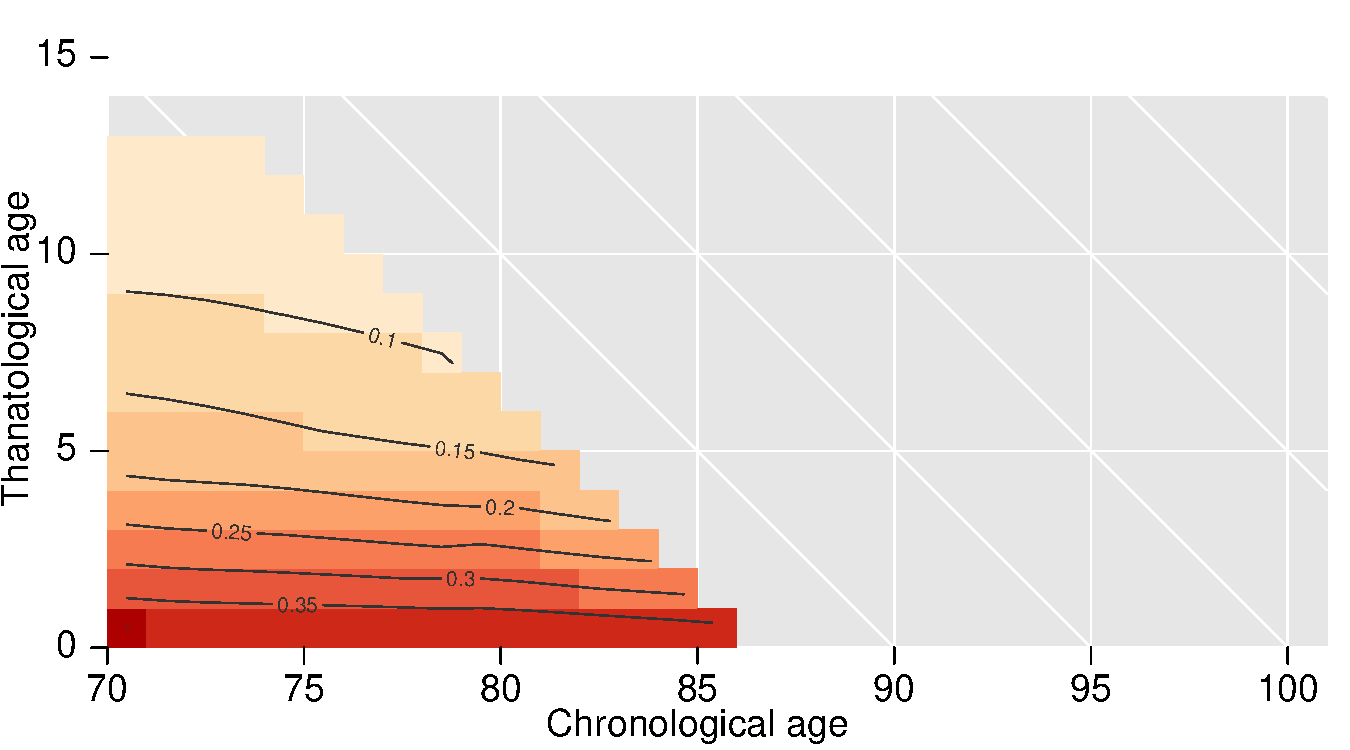
\includegraphics[scale=0.25]{Fig7e.pdf}
%\end{subfigure}
%~
%\begin{subfigure}{.46\textwidth}
%\centering
%\caption*{~}
%\label{fig:srhlegend}
%%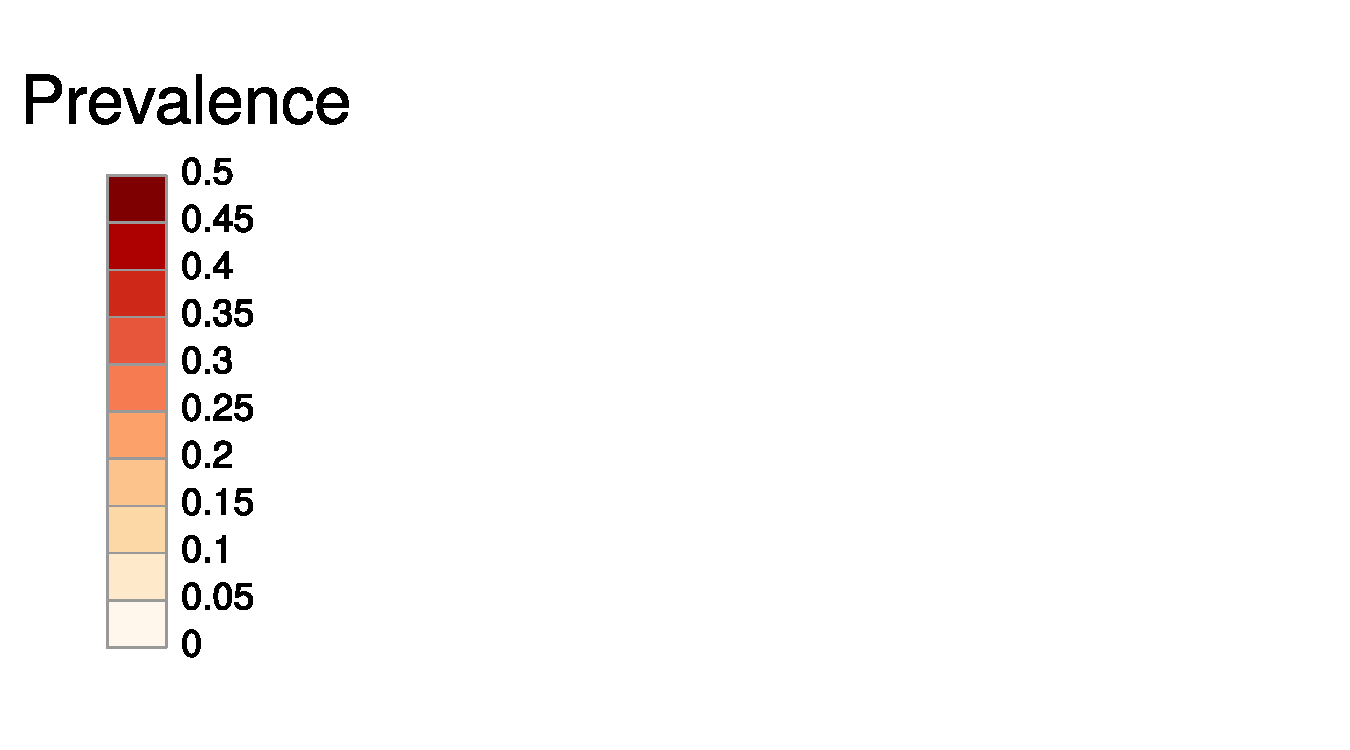
\includegraphics[scale=0.25]{Fig7Legend.pdf}
%\end{subfigure}
%\end{figure} 

Figure~\ref{fig:poorsrh} displays a series of TAL surface plots of male
SRH prevalance, each referring to a different quinquennial birth cohort (1905--09, 1910--14, $\dots$). These follow the coordinates of the TAL diagram in Fig.~3.
The $x$-axis is chronological age, the $y$-axis is thanatological age, and
downward-sloping diagonals delineate lifespan. Lifelines (not drawn) descend
parallel to the downward diagonals seen on the background grid. The density of
lifelines in each surface is not visible in this rendering, but one can imagine
the mode of the lifetable deaths distribution running down the diagonal that
meets near age 80 on the $x$-axis. Each surface describes the end-of-life SRH
prevalence of a birth cohort for the range of lifespan permitted by the survey,
but with a lower bound of 70 and an upper bound of 100. Surfaces are therfore
shifted down five ages (leftward) for each successive quinquennial birth cohort.
Colors and contours indicate prevalence value ranges, with pastel pink for low
values (under 10\%) and deep reds for high values (over 40\%).

 Contour lines in the surfaces are perpendicular to the primary direction of
 variation.
 For each cohort, the deepest red bar is located in the last
 year of life and spread over a wide range of ages, giving a roughly horizontal contour line.
Other contour lines are also relatively horizontal. This means that variation
(in this window of observation) is mainly over thanatological age and not over
chronological age. Were variation mostly a function of chronological age the
contour lines would be vertical. For each of these birth cohorts we have a series of prevalence trajectories---
empirical examples of the lifeline morbidity trajectories often conceptually
diagrammed in the literature on morbidity compression
\citep[e.g.,][]{fries2005frailty}. If we were to summarize each of
these surfaces with a single line, a thanatological age pattern would give a
much more compact description than a chronological age pattern. Patterns are
also relatively stable between cohorts.

When weighted by lifelines, the marginal chronological age pattern of SRH,
i.e. as measured with the ``Sullivan curve'' \citep{Sullivan1970}, would show an
increasing tendency over age, in agreement with common expectations.
However, such an increasing pattern over age is a marginal artifact, due to an
interaction between the distribution of lifespans and the relatively fixed underlying
pattern of morbidity seen in Fig.~7. These surfaces can indeed
be tidily summarized with a single line, but it is a line over the
thanatological age margin rather than over chronological age. 

Since the patterns for each of these cohorts can be presumed to be the same, any
shifting in the distribution of age at death ought not produce a change in the
expected years of poor health for a given length of life. Further, cohort
expected life years spent in poor health should also be approximately the same,
even if the underlying age-at-death distribution shifts upward. If morbidity
change is a pure function of thanatological age, an increase in life expectancy
should increase healthy life expectancy by the same amount. This is not the
prediction when we base analyses on the chronological age pattern of
self-reported health. Indeed, an underlying morbidity pattern as stable as
that seen in Fig.~7 would predict improvements in the marginal
chronological age pattern of self-reported health if the lifespan distribution
were to shift to higher ages. This is because a higher age at death implies
more years lived in ages farther from death, where prevalence is low.
This potential bias in the current status quo of morbidity measurement and
prediction leads to pessimistic morbidity scenarios when mortality improvements
are projected, and it undermines health expectancy comparisons between groups
with different mortality \citep{vanRaalte2015HLE}.
Cohort health expectancies are in either case unbiased, but these are also not
commonly estimated due to data constraints. This approach and essential finding
is in agreement with the results of similar analytic approaches to the
prediction of healthcare expenditure
\citep[e.g.,][]{miller2001increasing,Geue2014}

Using the data from our example surfaces, we calculate some basic results that support our case. Let us take the population of US males aged 60 and older, and
assume that mean time-to-death trajectory derived from the
Fig.~7 surfaces is valid for them.
We apply this trajectory to the synthetic stationary population of each
year from 1980 and 2010 \citep{HMD} following the formulas in
\cite{vanRaalte2015HLE}. We then calculate the resulting healthy and unhealthy
life expectancies, and compare these with expectancies calculated using the
standard Sullivan method and assuming the 1980 chronological age
pattern of poor SRH.\footnote{The 1980 chronological age pattern of poor SRH is
calculated from the 1980 stationary population and the same fixed time-to-death
prevalence trajectory.} Total remaining life expectancy at
age 60 increased 4.3 years from 17.4 in 1980 to 21.7 years in 2010.
Assuming the time-to-death prevalence trajectory, we calculate
healthy life expectancies of 15.7 and 19.9, respectively, an increase of 4.2 years. Unhealthy life expectancy in this scenario increased just 0.1 years. Had we used the Sullivan curve from 1980 to
calculate the 2010 values, we would have predicted an increase of 0.7 years in
unhealthy life expectancy, or 39\% versus the 4\% ``observed'' in this simple
scenario.

This is a large difference in projected morbidity, and it is based on a
relatively minor tweak to standard methodology, itself inspired by viewing data under the conditions
enabled by the demographic time framework and adjusting standard demographic
methods to capture the direction of temporal variation in data. There is a wide variety
of prevalence patterns when viewed in this way \citep{riffe2016ttd,
wolf2015disability}, and much empirical and methodological work is still required to verify
that these findings are representative and to understand the consequences for
the standard ways of comparing and projecting HLE. Our objective in this application has been
to demonstrate how viewing data structured by the
time-framework we propose can lead to new understandings and approaches to
processes over the life course. Other methodological applications of this
framework are imaginable in other phases of the life course, or non-human
subjects.

\section{Conclusions}

The age-period-cohort relationship is a special subset of a richer and unbounded
set of potential time identities. Of this infinite set of
temporal relationships, we present one six-way demographic time
identity that expands the Lexis diagram to a Lexis ``space'' so as to structure
transitions with respect to both birth and death (entry and exit). We call this
hexad relationship a demographic time framework because it is based on
the events of birth and death in calendar time, entailing six time measures:
chronological age (A), period (P), birth cohort (C), time to death (T), death cohort (D), and individual lifespan (L). In
Sect.~\ref{sec:dyads2diagrams} we show how combinations of these time measures imply four triad identities, each of which consists in simple linear relationship between its three
constituent time measures. We describe how each triad identity can be
extended into a temporal plane, with a characteristic diagram. The four triad
identities underly a family of four diagrams that include the
familiar Lexis diagram, but also three either new or
uncommon diagrams: The TPD, which is a sort of dual to the Lexis diagram; the TAL, whose use we deomonstrate in Sect.~\ref{sec:app}; and the LCD diagrams.

These four identities and diagrams relate to one another in a single
relationship that can be represented in 3-dimensional space. 
In Sect.~\ref{sec:diagram} we render a diagram of the demographic time
identity. We argue that the full three dimensional diagram is not necesarily a
practical way to represent demographic data, but that it forms a useful
reference to understand demographic structure. Practically, data structured by
all six demographic time measures can be represented on any of the four diagrams
if controlled properly. In Sect.~\ref{sec:app} we present a brief
application of this technique to the prevalence of poor self-reported health in
older ages in the United States.  We show that the choice of age pattern when calculating
prevalence-based measures of healthy life expectancy can have a large impact on
healthy life expectancy. The size of the effect varies depending on the morbidity pattern, and on how fast mortality and
morbidity are both changing. However, the experience of old-age mortality
improvement in recent decades leads us to suspect that many projections of
old-age morbidity burden are likely to be needlessly pessimistic if it is the
case that the prevalence of pertinent health conditions varies primarily as a
function of time to death. This clearly merits further study in the case of human population
health, and we speculate that findings of similar import may arise if
this framework is used to visualize data and inform new methods in other
unrelated areas of investigation.

In Sect.~\ref{sec:gen} we digress to present a more general event-duration identity framework, which allows us to situate the demographic time hexad identity more
rigorously as a special case of an event-duration framework. We compare this
identity with other relatively complicated temporal relationships in the literature, including the \citet{lexis1875einleitung}
marriage identity and the illness-death model by \citet{brinks2014lexis}. Our comparison between complex statistical designs serves to illustrate the
transferability of the concepts we present to other applications. The
examples we select to illustrate this framework happen to be from social and
medical sciences, but the same relationships hold in any single or multi-state
situation. That is to say, one may represent the time-space of any phenomenon,
transition, dated event, or sequence thereof by deriving the time identity graph
as in Table~\ref{tab:timelines} and using this as the basis of further
analysis. 
%Some general properties of temporal identities are given in
%Sect.~\ref{sec:gen}. In Sect.~\ref{sec:tetrahedron} we describe how the graph
% of the demographic time identity is also the graph of a tetrahedron. As a three-dimensional solid, the tetrahedron forms the basis of the three dimensional extension of the demograhic time identity. Each of the four faces of the tetrahedron is parallel to one of the four temporal planes. The same relationship between planes and the 3d space would hold for all other
%temporal hexad identities as well.

Data visualization is an effective way to detect patterns in temporal variation. The generalized time framework we propose is conceived as one
adequate to capture all possible temporal variation. The demographic time hexad identity is a special case whose use we suggest for
visualizing macro patterns in demographic data, probably via small multiples of
successive time slices in one of the diagrams from Sect.~\ref{sec:dyads2diagrams}, similar to that shown in Fig.~\ref{fig:poorsrh} on the basis of the TAL diagram.
Such visualization strategies at this time are exploratory, and this is a
technique that may benefit from further refinement. Further, a cross-section
through the demographic time-space need not be parallel to one of the four
identity-planes. Other more complicated temporal designs are also possible,
potentially based on even higher dimensional time-spaces. In this case,
cross-sections may also be a helpful trick for visualization, although this is
an area in need of future work. Further, if the purpose of visualization in
this case is merely to detect the principal direction of variation, appropriate
statistical methods should be developed (or recommended) to do so in a more
rigorous way, and these should be flexible with respect to the full set of time measures implied by a given
identity.

Several lines of substantive research may be augmented by or based on the
findings we present. For example, it is of public health interest to document
the full range of late-life morbidity patterns over various time measures. We do
not at this time know how the late life morbidity patterns referred to in
Sect.~\ref{sec:app} change over time or vary between populations, for example.
This has implications for the use of health expectancies and related measures in comparative studies of disease burden.
However, the time framework we describe may also be useful more generally to
structure disease processes. More broadly, the temporal dynamics of classiscal
demographic processes such as childbearing, partner formation and dissolution,
migrations, employment transitions, and temporal interactions between these events may also be fully captured and explored under our framework. To do so, we
offer some tentative advice: First create the identity graph of interest; next
complete the data to include ``implied'' time measures; then toggle through
cross-sections of the structured data to determine which ones reveal important patterns.
The phenomena that we are most likely to learn the most about by taking this
simple analytic step are those that are dogmatically held to vary only over age.

Finally, we believe in the pedagogical value of the framework
introduced in this paper. We hope that the
present inquiry will be useful as a teaching instrument in the same way as Lexis
diagrams have formed a part of basic demographic education.
Our generalized time framework and the relationship between the six dimensions
of demographic time both help situate the APC paradigm in a broader context.
Just as scientific discovery in general depends partly on the development of
finer optics and instrumentation, we hope that the framework we describe will prove an instrument to enable new discoveries in formal and empirical demography, as well as other diverse fields of
investigation.

%\nocite{oreg,schn,pond,smith,marg,hunn,advi,koha,mouse}

%%%%%%%%%%%%%%%%%%%%%%%%%%%%%%%%%%%%%%%%%%%%%%
%%                                          %%
%% Backmatter begins here                   %%
%%                                          %%
%%%%%%%%%%%%%%%%%%%%%%%%%%%%%%%%%%%%%%%%%%%%%%

\begin{backmatter}

%\section*{Competing interests}
%  The authors declare that they have no competing interests.

%\section*{Author's contributions}
%    Text for this section \ldots

%\section*{Acknowledgements}
%  Text for this section \ldots
%%%%%%%%%%%%%%%%%%%%%%%%%%%%%%%%%%%%%%%%%%%%%%%%%%%%%%%%%%%%%
%%                  The Bibliography                       %%
%%                                                         %%
%%  Bmc_mathpys.bst  will be used to                       %%
%%  create a .BBL file for submission.                     %%
%%  After submission of the .TEX file,                     %%
%%  you will be prompted to submit your .BBL file.         %%
%%                                                         %%
%%                                                         %%
%%  Note that the displayed Bibliography will not          %%
%%  necessarily be rendered by Latex exactly as specified  %%
%%  in the online Instructions for Authors.                %%
%%                                                         %%
%%%%%%%%%%%%%%%%%%%%%%%%%%%%%%%%%%%%%%%%%%%%%%%%%%%%%%%%%%%%%


% if your bibliography is in bibtex format, use those commands:
% \bibliographystyle{bmc-mathphys} % Style BST file (bmc-mathphys, vancouver, spbasic).
\bibliographystyle{chicago}
\bibliography{references}      % Bibliography file (usually '*.bib' )
% for author-year bibliography (bmc-mathphys or spbasic)
% a) write to bib file (bmc-mathphys only)
% @settings{label, options="nameyear"}
% b) uncomment next line
%\nocite{label}

% or include bibliography directly:
% \begin{thebibliography}
% \bibitem{b1}
% \end{thebibliography}

%%%%%%%%%%%%%%%%%%%%%%%%%%%%%%%%%%%
%%                               %%
%% Figures                       %%
%%                               %%
%% NB: this is for captions and  %%
%% Titles. All graphics must be  %%
%% submitted separately and NOT  %%
%% included in the Tex document  %%
%%                               %%
%%%%%%%%%%%%%%%%%%%%%%%%%%%%%%%%%%%

%%
%% Do not use \listoffigures as most will included as separate files

\section*{Figure captions}

% Fig1
\begin{figure}[h!]
  \caption{\csentence{An APC diagram with six lifelines.}}
  \label{fig:APC}
\end{figure}

% Fig2
\begin{figure}[h!]
  \caption{\csentence{A TPD diagram with six lifelines.}}
  \label{fig:TPD}
\end{figure}

% Fig3
\begin{figure}[h!]
  \caption{\csentence{A TAL diagram with six lifelines. Since two of the six lifelines are
 of equal length (75), they are overlapped in this figure and appear to be five.}}
\label{fig:tal}
\end{figure}

% Fig4
\begin{figure}[h!]
  \caption{\csentence{An LCD diagram with six lifelines. Since the LCD plane is orthogonal
to the life course, lifelines are depicted as points}}
  \label{fig:lcd}
\end{figure}

% Fig5
\begin{figure}[h!]
  \caption{\csentence{Tetrahedral graph of demographic time hexad identity, with edges
labelled by the six time indices.}}
\label{fig:tet}
\end{figure}

% Fig6
\begin{figure}[h!]
  \caption{\csentence{Diagram of the hexad identity, showing a sequence of TAL
planes intersecting with a single APC plane at the base.}}
\label{fig:apctTAL}
\end{figure}

% Fig7
\begin{figure}[h!]
  \caption{\csentence{Prevalence of males self-reporting poor health by chronological and
thanatological age, by quinquennial birth cohorts, 1905--1925 (Sources: \citealt{HRSumich, HRS})
}}
\label{fig:poorsrh}
\end{figure}
%%%%%%%%%%%%%%%%%%%%%%%%%%%%%%%%%%%
%%                               %%
%% Tables                        %%
%%                               %%
%%%%%%%%%%%%%%%%%%%%%%%%%%%%%%%%%%%

%% Use of \listoftables is discouraged.
%%
\pagebreak
\section*{Tables (1 given, 2 and 3 included separately)}

% Table 1
\begin{table}[h!]
\centering
\caption{Definitions of the six time measures.}
\label{tab:sixdefs}
\begin{tabular}{lll}
\hline 
\textbf{Time measure}	& \textbf{Demographic definition}	& \textbf{Event history definition}	\\ \hline 
A - chronological age 	& time since birth 			& time since start of exposure 		\\
P - period 		        & calendar time 			& calendar time				\\
C - birth cohort 	    & calendar time of birth 	& calendar time of exposure
start
\\
T - thanatological age 	& time until death 			& time until event			\\
D - death cohort	    & calendar time of death	& calendar time of event		\\
L - lifespan		    & duration of life			& duration of exposure			\\ \hline
\end{tabular}
\end{table}

% table 2
\begin{longtable}{m{0.15\textwidth}L{0.5\textwidth}C{0.2\textwidth}}
  \caption{All dyadic juxtapositions of the six measures of
  demographic time.} \label{tab:dyads}\\
 
  \toprule
  \multicolumn{3}{m{0.9\textwidth}}{\footnotesize \emph{Note:} The temporal
  planes are named after the two given time scales. The derived scale is appended in parentheses. Contrary to mathematical convention we name the ordinate scale first and the abscissa scale second. This is to be consistent with the established APC and ACP terms.} \\

\end{longtable}

% table 3
\begin{table}[h]
\centering
\caption{Event-duration timeline and graph for two, three, and four event sequences.}
\label{tab:timelines}
\end{table}


%%%%%%%%%%%%%%%%%%%%%%%%%%%%%%%%%%%
%%                               %%
%% Additional Files              %%
%%                               %%
%%%%%%%%%%%%%%%%%%%%%%%%%%%%%%%%%%%

%\section*{Additional Files}
%  \subsection*{Additional file 1 --- Sample additional file title}
%    Additional file descriptions text (including details of how to
%    view the file, if it is in a non-standard format or the file extension).  This might
%    refer to a multi-page table or a figure.
%
%  \subsection*{Additional file 2 --- Sample additional file title}
%    Additional file descriptions text.


\end{backmatter}
\end{document}
